\documentclass[a4paper,titlepage]{article}


\usepackage{listings}
\usepackage{caption}
\usepackage{graphicx}
\usepackage{geometry}
\usepackage{changepage}
\usepackage{titling}

\geometry{verbose,tmargin=2.5cm,bmargin=2.5cm,lmargin=2.5cm,rmargin=2.5cm}

\title{Community Detection based on Modularity on the GPU}
\author{Fontolan Federico}


\begin{document}
	\begin{titlepage}
	\newgeometry{margin=2cm}
	\includegraphics[width=0.25\textwidth]{0-resources/logo_ca_foscari.png}
   \begin{center}
       \vspace*{2cm}
       \textbf{Master’s Degree \\
       	in Computer Science}
 
       \vspace{2cm}
       \textbf{Final Thesis}
 
       \vspace{1cm}
		\textbf{\Large\thetitle}
   \end{center}

	\begin{adjustwidth}{0.7cm}{0cm}
		\vspace{3cm}
		\textbf{Supervisor}\\
		Ch. Prof. Claudio Lucchese
		
	
		\vspace{0.5cm}
		\noindent\textbf{Graduand}\\
		Federico Fontolan
		
		
		\vspace{0.5cm}
		\noindent\textbf{Matriculation Number}\\
		854230
		
		\vspace{0.5cm}
		\noindent\textbf{Academic Year}\\
		2019 / 2020
	\end{adjustwidth}
	
\end{titlepage}
	
	\begin{abstract}
		Modularity algorithms for the detection of communities are the de facto standard thanks to the fact that they offer the best result between efficiency and result. 
		Moreover these algorithms allow to analyze graphs much larger than those that can be analyzed with alternative techniques. Among these the Louvain algorithm has become extremely popular due to its simplicity, efficiency and precision.\\
		In this thesis will be presented an overview of community detection techniques and a new parallel implementation of the Louvain algorithm written in CUDA and exploitable by Nvdia GPUs.
	\end{abstract}

	\tableofcontents
	\newpage
	
	\section{Introduction}
The community detection problem is one of the most interesting fields of graph analysis. In several real-world scenarios, we have the necessity of cluster some data considering the relations between them: one example can be the problem of dividing social network users in groups by the mutual friendship relations to propose targeted advertisings. A natural way to represent this kind of structure based on the relation is a graph, and several techniques based on this theory was proposed in the literature to solve this kind of problem. This problem is not easy to solve due to the extremely high number of different possible partitions of the data that we can perform, even if the dataset is composed of few elements.
One the most famous and used heuristic is the Louvain algorithm proposed by Blondel et al. \cite{Blondel_2008}, due to its speed and its overall quality, even if its limits are well known in the literature. This greedy algorithm divides the graph into partitions maximizing a quality function that evaluate them, called \textbf{modularity}. This function is based on the idea that a random graph doesn't exhibit a community structure: therefore, we can evaluate how is well defined the community structure comparing the graph with another graph that keeps some of its structural proprieties but is generated at random, called \textit{null-model} \cite{Girvan2002Community}. Given a graph $G(V,E)$, its adjacency matrix $A$, a partition of nodes $C$ and the corresponding function $c(x)$ that assign each node $x$ to its community, we define the modularity function as follow:
\begin{equation}\label{intro_Q}
Q = \frac{1}{2|E|} \sum_{i,j \in V}\left(A_{ij} - \frac{k_ik_j}{2|E|}\right) \delta(c(i), c(j))
\end{equation}
where $k_i$ is the degree of the node $i$ and $\delta$ is an filter function: its yields one if $c(i) = c(j)$, zero otherwise.
The techniques proposed before the Louvain algorithm are quite slow because, every time we assign a node to a community, we have to recalculate the values with the previous formula, and this calculation takes a lot of time. To speed up the computation, this algorithm proposed to calculate the variation in modularity assigning a node to another community without recalculating $Q$ with the Formula \ref{intro_Q}. The algorithm is composed of two phases: an optimization phase and an aggregation phase. At the beginning each node is assigned to a community composed only by itself; in the first, we pick each node $i$ of the graph and we calculate for each community $c_j$ in its neighbourhood the values $\Delta Q_{i \rightarrow c_j}$, that is the changing in the modularity of assigning the node $i$ to the community $c_j$, as following:
\begin{equation}\label{intro_Delta}
\Delta Q_{i \rightarrow c_j} = \frac{l_{i\rightarrow c_j} - l_{i\rightarrow c_i / \{i\}}}{2|V|} + k_i \frac{k_{c_i / \{i\}} - k_{c_j}}{4|V|^2}
\end{equation}
where $l_{i\rightarrow c_j}$ is the sum of edges that connect $i$ to the community $c_j$, $k_i$ is the weight of the nodes $i$ and $k_{c_j}$ is the weight of the community $c_j$. Then, for each node, we select the maximum values and if it is greater than zero, we assign the node $i$ to the community that corresponds to the maximum value. We repeat this procedure sequentially for all nodes while the modularity score increases. When no more improvement can be achieved, we execute the aggregation phase. In this phases we create a new graph from the current community structure: each node is one of this communities, and the edge between them is given by the sum of the links between nodes that belong to the corresponding communities (edge between nodes in the same communities lead to self-loop). After this step, we reapply the first step. The algorithm ends up when no more improvement is obtained.
This algorithm is quite efficient with a complexity of $O(m)$ where $m$ is the number of edges in the graph, but this algorithm requires a lot of time to find the communities in the bigger graphs. For this reason, some approaches were proposed in the literature to speed up the algorithm. One interesting technique proposed by Ozaki et. al \cite{pruning}, prune the nodes in the optimization phase, considering only the nodes that have a neighbour that has to change its community in the previous iteration. Apart from this kind technique, generally, the most effective method to improve significantly the performance of an algorithm is to parallelize the execution. Especially, to obtain the maximum speed, many frameworks that allow performing on the GPU computation normally handled by the CPU became popular. The most used framework is the Nvidia CUDA, a parallel computing platform and application programming interface. CUDA was originally designed as a C++ language extension that allows any developer to building application designed for the GPU with a low learning curve. CUDA is also designed to transparently scale on different GPU.\\
In literature, several implementations of the Louvain algorithm for the GPU were proposed. In this thesis, we present three new algorithms for the GPU based on the Louvain algorithm: PSR-Louvain, PH-Louvain and Adaptive Louvain. All these algorithms implement the pruning techniques proposed by Ozaki. No other Louvain based algorithm for the GPU implements this technique before. 
These algorithms compute the maximum score of $\Delta Q$ for each node simultaneously, and then we update the community based on that score. Also, the creation of the edges of the new graph in the aggregation phase is executed in parallel. 
The first two algorithms are quite similar to each other. In both algorithm we start from the edge list composed by the tuple $(i,j,w)$ where $i$ is the source node of the edge, $j$ is the destination node of the edge and $w$ is the weight of the edge.
Both algorithm, in the optimization phase, first select only the edges such that the node $i$ has a neighbour that has to change its community in the previous iteration, then they substitute each destination node with the corresponding community $c_j$. After them, the two algorithms using different methods to sum up all the values $w$ for each pair $i$ and $c_j$ and obtain the corresponding $l_{i\rightarrow c_j}$. We need this value to compute all the $\Delta Q_{i \rightarrow c_j}$, as shown in the Formula \ref{intro_Delta}. The first algorithm sorts the list and then performs a segmented reduction to each value with the same pair $i$ and $c_j$; the second algorithm use a hashmap to aggregate all of these values. After then, both select the maximum value for each node and eventually update the community. Finally, they compute if a node has a neighbour that change its community and store the results that will be used in the next iteration for the pruning. These two algorithms use the same aggregation scheme proposed in the optimization phase to create the new graph in the aggregation phase. In both algorithm is also present a technique that optimizes the first iteration of each optimization phase. \\
This two algorithm, compared to the fastest sequential versions, obtain a speed-up factor up to 56.
During the analysis of this two algorithm, we discover that the PSR-Louvain tends to perform better than the PH-Louvain in the early iteration of the optimization phase; on the other hand, the PH-Louvain approach outperforms the other when the number of a different key inserted in the hashmap falls below a given threshold. Besides the PH-Louvain aggregation phase is faster than the PSR-Louvain one. \\
On these considerations, we create a new algorithm that combines these two algorithms and selects the best aggregation scheme on the situation. This Adaptive approach performs better than the other, combining effectively the best feature of these two algorithms. Finally, we compare this version with the two fastest GPU Louvain based algorithm: the first one is included in the Nvidia library cuGraph; the second one is included in the high-performance library for graph analysis Gunrock. Our test highlight that our Adaptive algorithm optimizes the memory occupation better than the other two allowing it to compute graph with approximately twice edges. Besides, our algorithm generally perform better than these two algorithms in terms of time.\\
This thesis is structured as follows:
in Chapter \ref{C2} of this thesis, we present the Nvidia GPUs architecture and the CUDA framework, paying special attention to the concept that is used later on this thesis; in the Chapter \ref{C3} we present the field of the community detection and the modularity optimization, highlighting the motivation that leads to the design of the Louvain Algorithm; in the Chapter \ref{C4} we present the sequential Louvain algorithm, the pruning techniques and the previous parallel implementations presented in the literature;
then, in Chapter \ref{GPUalg}, we present in details our two first algorithm, that will be analyzed in details in the Chapter \ref{C6}; finally, in the Chapter \ref{C7}, we present the Adaptive Louvain algorithm and we analyze it, comparing it first with our other two algorithms, then with the two algorithms included in the two libraries. In the last chapter, we sum up our work and we highlight some future research areas and development.
	
	\section{Community Detection State of the Art}
\begin{figure}[h]
	\centering
	\includegraphics[width=0.6\linewidth]{0-resources/community1}
	\caption{An example of a communities structured graph. Three communities are enclosed by the rectangles.}
	\label{fig:community1}
\end{figure}
\noindent The problem of community detection raises in many application scenarios from the necessity of finding groups of objects that have a large number of connections to each other. To represent problems where it is fundamental to empathize connection between objects, the graph theory is the main tool. A graph is a mathematical structure composed of nodes (or vertices) that denote the objects and edges (or links) that express some kind of relationship between objects and possibly having a weights that quantifies this relationship.
The Graph Theory born in 1736 when Euler used this mathematical abstraction to solve the puzzle of Königsberg’s bridges. Since then, this tool was used in several of Mathematics, Social, Biological and Technological application. In recent time, the approach to this studies has been revolutionized to deal with bigger and more complicated challenges, supported by the increasing computing power.
\begin{figure}[h]
	\centering
	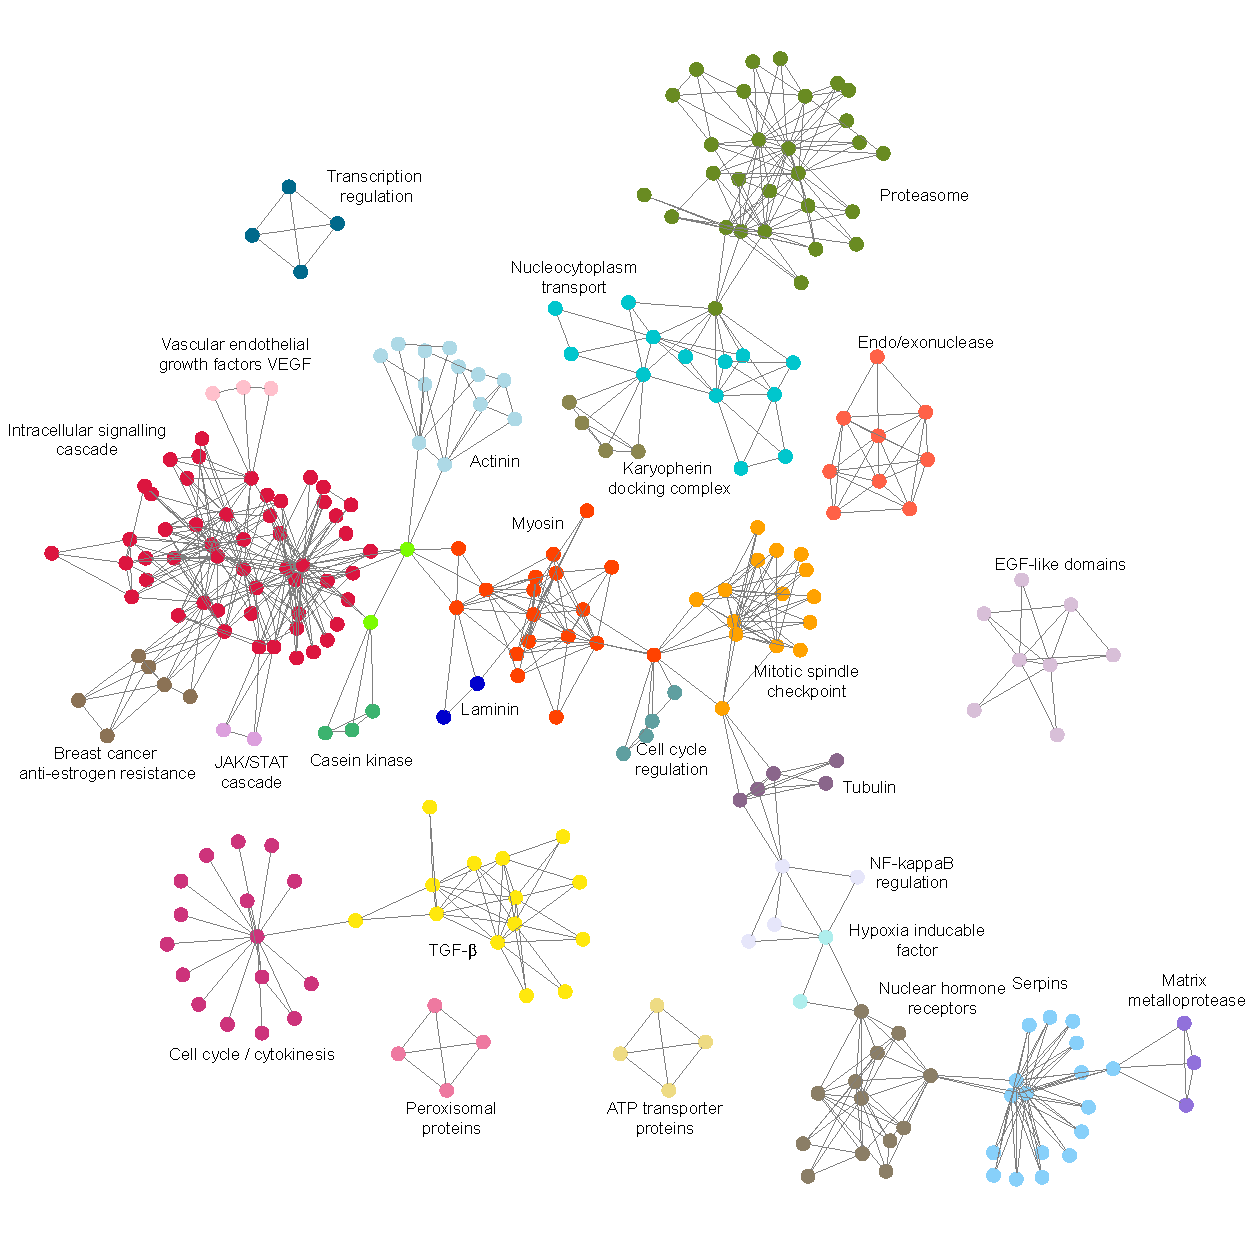
\includegraphics[width=1\linewidth]{0-resources/ppi}
	\caption{A protein protein iteration network of a rat cancerous cell. This image was reprinted from \cite{metastasis}.}
	\label{fig:ppi}
\end{figure}\\
The necessity of finding this high-connected substructure in graph arises from real problems in different research areas: for example, the study of Protein-Protein Interaction (PPI) networks is very important because the interaction between proteins is the basis of all process in the cell.\\ A study demonstrated that this type of network shown to be useful for highlighting key proteins involved in metastasis. \cite{metastasis} \\
Other examples can be found in the field of sociology: a historically well-know scenario is the Zachary's Karate Club. This dataset captures members of a Karate Club for 3 years.\cite{Zac77} An edge between two nodes represents an interaction between two members outside the club. At some point, a conflict between the administrator and a master led to split of the club into two separate groups. The question is if it is possible to infer who compose these two new groups basing on the information that this graph give to us. 
\begin{figure}
	\centering
	\includegraphics[width=0.6\linewidth]{0-resources/karateclub}
	\caption{Zacahry's karate club. \cite{Zac77} This image was made with Graphviz.}
	\label{fig:karateclub}
\end{figure}
This small network of 1977 is famous because it has often been used as a reference point to test the detection algorithms used to analyze huge social web networks.
In general this kind of problem, i.e. clustering people that belong to the same community base on interaction, it's useful not only in sociology but also in marketing: by knowing people with similar interests, it's possible to make better recommendation systems.\\
There are several of similar real-world scenarios, all united by the fact that the data is unregular but it's present some well-defined topological structure that in a completely random graph are absent. A random graph is a fully disordered graph, firstly proposed by Erdös and Rényi \cite{random} in 1959: it's a graph where the probability that there is an edge between two nodes it's equal for all pairs of nodes and, for this reason, the degree of the nodes (i.e. the number of edges incident to a node) is homogeneous. In real networks, this is not true, because they are often scale-free (follow a power-law distribution). An example of this is the study about the citations in scientific papers made by Derek J. de Solla Price in 1965 \cite{dsp} or the study about World Wide Web growing made by Albert-László Barabási et al in 1999 \cite{Barab}.
Furthermore, the degree distribution of the nodes is non-homogeneous not only globally but also locally, this due to the observation that there is a high concentration of edges within sets of nodes and a low concentration of edges between this sets. These two concepts are essential to formulate the formal definition of Community and Modularity. In this chapter will be presented some definitions of community and will be given an overview of some methods that are used to identify communities.
\subsection{Community Definitions}\label{3.1}
The informal definition of community is there are many more edges inside the community versus the rest of the graph, but there isn't a unique quantitative definition of community. This kind of freedom is necessary because the concept of community is strictly connected to the problem that will be analyzed: for example, in some cases, it's necessary that communities overlap, but in other problems, this is not necessary. There is a unique key constraint that allows talking about community detection: the graph must be sparse. A sparse graph is a graph where the number of nodes has the same magnitude of the number of edges. In the unweighted graph case, if the number of edges is far greater than the number of nodes, the distribution of edges among the nodes is too homogeneous for communities to make sense \cite{fortunato}. In that case, the problem nature is little different: we aren't interested anymore on the edge density between nodes but we have to use some kind of metrics (like similarity or distance) to clustering. In that case, the problem is more similar to data clustering. Despite this, assuming that a community is a subset of similar nodes it's reasonable, for this reasons some techniques (like spectral o hierarchical clustering) belonging to this field are adopted in community detection and will be shortly presented later on this thesis.
Following this, Fortunato \cite{fortunato} defines three main classes of community's definitions: \textit{local, global and based on vertex similarity}. Other types of definitions are still possible, but these three offers give a good summary of the problem. We now present those classes to give an overview of the various approach that has been used to define this problem. 
\subsubsection{Local definitions}\label{local-def}
Considering that a community has a lot of interactions with the other nodes that are in it and few connections outside, it is fair to think about the communities as autonomous objects.
The local definitions are based on this concept. Directly from this concept, we can think at the community as a clique, i.e. a subset whose vertices are all adjacent to each other. This type of definitions it's too strict: even if just one edge is not present, the subset is not a clique, but the subset has a very high concentration of edges. For this reason, the clique definition is often relaxed, using, for example, $n$-clique, i.e. a subset in which all the vertices are connected by a path of length less than $n$.\\
Anyway, this type of definitions ensure that there is a strong cohesion between the nodes in the subset, but it does not ensures that there isn't a comparable cohesion between the subset and the rest of the graph. For this purpose, other definitions were proposed. 
Given a graph $G(V,E)$, the corresponding adjacency matrix $A$ and a subset of nodes $C$ where $C \in V$, we define the internal degree $k_v^{int}$ and the external degree $k_v^{ext}$ for each vertex $v$ that belongs to $C$ as the number of edges that connect the node $v$ with another node that belongs to $C$ and not belongs to $C$, respectively:
\begin{align}
k_v^{int}= \sum_{k \in C} A_{vk} && k_v^{ext}= \sum_{k \notin C} A_{vk}
\end{align}
where $A_{vk}$ is the entry of $A$ at position $(v,k)$. We also define the internal degree $k_C^{int}$ and the external degree $k_C^{ext}$ as the sum of all internal and external degree of nodes that belongs to $C$. 
\begin{align}
k_C^{int}= \sum_{i,j \in C} A_{ij} && k_C^{ext}= \sum_{i\in C, j \notin C} A_{ij}
\end{align}
A strong community is a subset of nodes such that the internal degree $k_n^{int}$  for each vertex $n$ is greater than its external degree $k_n^{ext}$ . This type of definitions once again very strict, for this reason we define as weak community a subset of nodes where the internal degree of the subset  $k_C^{int}$ is greater than its external degree $k_C^{ext}$. Many other variants of these definitions were presented in the literature.
\subsubsection{Global definitions}
The previous class quantifies the communities independently, considering every subset individually. Overturning the point of view, we can define communities in a graph-dependent way, considering them as an essential and discriminant part of it. There are many different interpretations of this approach in the literature, but the most important definitions are focused on this key fact: it's not expected to see a community structure in a random graph. For this reason, we define as \textit{null model} of a graph another graph that has some features in common with the original one but it's generated randomly. This graph is used as a comparison term to identify if it's present a community structure in the graph or not and, if it is present, to quantify how it is pronounced.
The comparison between a graph and the corresponding null model, which is based the Modularity Optimization, is the main object of this study and is presented in detail in the next chapter.
\subsubsection{Based on Vertex Similarity}
The last class of definitions assumes that edges in the same community are similar to one another. All the definition used in the classic clustering methods belongs to this class because they calculate a distance (similarity) between object and aren't based on the edge density like the previous definitions. This distance can be calculated in various ways:  if it is possible to embed the vertices into a $n$-dimensional Euclidean space by assigning a position to them, one method consists to calculate the distance between two nodes, considering that similar vertices are expected to be close to each other. To calculate the distance, one could use a norm. Three norms often used in the literature are the following. Given two points $a=(a_1, ... , a_n)$ and $b=(b_1, ... , b_n)$ that belongs to the $n$-dimensional Euclidean space $E$, we define the norms $l_1$ (Manhattan distance), $l_2$ (Euclidian distance) and $l_3$ (Maximum distance) as:
\begin{align}
l_1(a,b) =&\sum_{k=1}^{n} |a_k - b_k|\\
l_2(a,b) =&\sum_{k=1}^{n} \sqrt{(a_k -b_k)^2}\\
l_3(a,b) =&\max_{k \in [1,2]} |a_k - b_k|
\end{align}
Another option is the cosine similarity $\cos(a, b)$, that is very popular in literature:
\begin{equation}
\cos (a,b) = \frac{ \sum_{i=1}^{n}{{a}_i{b}_i} }{ \sqrt{\sum_{i=1}^{n}{({a}_i)^2}} \sqrt{\sum_{i=1}^{n}{({b}_i)^2}} }
\end{equation}
If it is not possible to embed the graph in a Euclidean Space, it is possible to infer the distance from the adjacency matrix. 
If it is not possible to embed the graph in a Euclidean Space, it is possible to infer the distance from the adjacency matrix. One idea is to map the distance in order to assign smaller values at nodes with the same neighbourhood. Given an adjacency matrix $A$ we define the distance between two nodes $a$ and $b$ as:
\begin{equation}
d(a,b) = \sqrt{\sum_{k\ne a,b} (A_{ak} - A_{bk})^2} 
\end{equation}
Many other variants of that definition (but based on the same principle) were presented in the literature, for example considering the overlap between neighbourhood respect to the union. \\
Other alternative measures consider the number of independent paths between nodes, i.e. path that does not share any common edges, or they are based on random walk on a graph: for example, the average number of steps needed to reach one vertex from another by a random walker.  

\subsection{Community Detection Algorithms}
A partition is a division of the graph in clusters, such that each vertex belongs to exactly one cluster. 
The partition of possible partitions of a graph $G$ with $n$ vertices grows faster than exponentially with $n$,  thus making it impossible to evaluate all the partitions of a graph \cite{fortunato}. For these reasons, many techniques were introduced to find the most significant ones.
We now present an introduction to some classical class of techniques used in the field of community detection: Partitional clustering, Graph partitioning, Spectral clustering, Hierarchical clustering.  Moreover, the Girvan and Newman algorithm is presented later on: even if this method is a Hierarchical algorithm, this method firstly introduced the modularity function and it is presented separately. The goal of this chapter is to give a useful overview in order to get the differences with the Modularity optimization and empathize the motivations that led to the choice of the Louvain algorithm, one of the most used nowadays, especially for huge graphs. For this reason, all the methods that are presented in this thesis find a partition, as the Louvain methods. 
For the sake of completeness, we remark that in Fortunato's report \cite{fortunato}, that was mainly used to write this chapter, is presented an analysis of algorithms that found also overlapping communities (covers). 
\subsubsection{Partitional clustering}
Partitional clustering is a class of methods that find clusters from data points. The algorithms in this class embed the graph in a metric space as seen in chapter \ref{local-def}, and then calculate the distance between these new points.  The goal is to separate the points in $k$ clusters minimizing the distance between points and to the assigned centroids (i.e. the arithmetic mean position of all the points in the cluster). The number of clusters $k$ is given as input. The most famous technique is k-means clustering.
The objective function to minimize is the following:
\begin{equation}
\sum^k_{i=1} \sum_{x_j\in C_i} || x_j - c_i ||^2 
\end{equation}
where $C_i$ is the $i$-th cluster and $c_i$ is its centroid. This function quantifies the intracluster distance. 
At the start, the $k$ centroids are set far distance from each other. Then, each vertex is assigned to cluster with the nearest centroid and the centroid is recalculated.  Even if the method doesn't find an optimal solution and the solution is strongly dependent on the initial setup of the centroids, this method remains popular due to the quick convergence that allows it to analyze big graphs.
However, setting the apriori number of cluster $k$ is not simple to estimate that number,
especially in a large graph, and for this reason, it is often preferred algorithms that can automatically derive it. Moreover, the embedding of the graph in the Euclidean Space may be tricky and not reliable for some graphs.
\subsubsection{Graph partitioning} 
Given a graph $G(V, E)$ and a number $g$ of clusters, the problem of graph partitioning consists of creating a partition of nodes composed by $g$ subsets such that it minimizes the edges lying between the clusters. To archive this goal, many algorithms perform a bisection of the graph, even for partitions with more than two clusters, where the bisection is iterated.  One of the earliest and famous algorithms is the Kernighan–Lin algorithm. This algorithm performs an optimization of the function $Q = link_{in} - link_{between}$, where $ link_{in}$ is the number of edges inside the subsets and $link_{between}$ is the number of edges lying between them. The algorithm starts from an initial partition (randomized or suggested by the graph), and the algorithm performs a swapping between clusters for a fixed number of nodes pair to increase the value of $Q$. 
To avoid local maxima, some swaps that decrease $Q$ are kept. 
With some optimizations, the complexity of this algorithm is $O(n^2)$ where $n$ is the number of nodes.\\
Other techniques are based on the max-flow min-cut theorem by Ford and Fulkerson \cite{ford} and the minimization of cut-affine measures, like the normalize cut:
\begin{equation}
\Phi_N(C) = \frac{c(C, V/C)}{k_c}
\end{equation}
where $C$ is a subset of nodes, $k_c$ is the total degree of $C$ and $c(C, V/C)$ is the sum of all the edges lying between the subsets $C$ and $V/C$. \\
Like the previous class, specifying the number of clusters is the greatest limit of this class of algorithm. In additions, iterative bisecting can lead to not reliable clusters, because the sub-clusters are made breaking the previous ones:  in this way, the new subsets have vertices only from one of the "parent" cluster.  
\subsubsection{Spectral clustering}
Given a set of $n$ object $x_1 ,x_2, ..., x_n$ and the matrix $S$ of pairwise similarity function $s(x_1, x_2)$ such that $s$ is symmetric and non negative, we define as spectral clustering all methods that using the eigenvector derived from the matrix $S$ to cluster the data.
In particular, this transformation makes a change from the reference system of the object to another whose coordinates are elements of eigenvectors. This transformation is made to enhance the proprieties of the initial data.  After that, we can cluster the data using other techniques as $k$-means and obtain a better result. The Laplacian matrix is the most used in spectral clustering. Given a graph $G$ and its associated adjacently matrix $A$, we define the Laplacian matrix $L$ of the graph $G$ as:
\begin{equation}
L = D - A 
\end{equation}
where $D$ is the degree matrix, a diagonal matrix which contains information about the degree of each vertex. This matrix is used due to nice propriety: if the graph has $k$ connected components, the Laplacian of the graph will have $k$ zero eigenvalues.
In that case, the matrix can be organized in a way that displays $l$ square blocks along
the diagonal. When is it in this block-diagonal form, each block is at his turn a Laplacian matrix of one of the subcomponent.
In this situation,
there are $k$ degenerate eigenvectors with equal non-vanishing components in correspondence with the vertices of a block and zero otherwise. 
Considering the $n\times k$ matrix where $n$ is the number of nodes of $G$ and the columns of this matrix are the $k$ eigenvectors, we can see that vertices in the same connected component of the graph coincide.
If the graph is connected but the connections between the $k$ subgraph are weak, only one eigenvalue is zero. By the way, However, the lowest $k - 1$ non-vanishing eigenvalues are still close to zero and the vertex vector of the first $k$ eigenvectors still identify the clusters.\\
An application of these techniques is the spectral bisection methods: this algorithm combines ideas from spectral clustering and graph partitioning. 
Given the graph $G$ with $n$ nodes, the cut size $R$ of the bipartition of the graph is:
\begin{equation}\label{spec_bi_pa}
R = \frac{1}{4} s^TLs
\end{equation} 
where $L$ is the Laplacian matrix and $s$ is the $n$-vector that represents the affiliation of the nodes to a group (if the node $i$ belongs to the first group, the $i$-th entry of $s$ will be $1$, $-1$ otherwise).
$s$ can be writtens as $s= \sum_{i=0}^n a_i v_i$ where $v_i$ is the $i$-th eigenvector of the Laplacian.
If $s$ is normalized, we can write the equation (\ref{spec_bi_pa}) as follows:
\begin{equation}\label{spec_bi_pa}
R = \sum_{i=0}^n a_i^2 \lambda_i
\end{equation} 
where $\lambda_i$ is the eigenvalue corresponding to $v_i$.
From this, choosing the $s$ parallel to the second-lowest eigenvector $\lambda_2$ we have a good approximation of the minimum because this would reduce the sum to $\lambda_2$. We remark that we use the second one because the first one is equal to zero. To cluster the data in the vector $s$, we match the signs of the components of $v$. \\
The exact computation of the all eigenvalues requires time $O(n^3)$, a too high complexity for big graphs, but there exist some techniques that allow calculating approximate values faster \cite{fortunato}.
 
\subsubsection{Hierarchical clustering}
The possible partitions of a graph can be very different in scale and some cluster in turn may show an internal community structure. In that case, there is a hierarchy between partitions. The most common way to represent this kind of structure is to draw a dendrogram, i.e. a diagram representing a hierarchical tree. If we draw an horizontal line in the dendrogram, observations that are joined together below the line are in the same cluster (Figure \ref{fig:dend}). The hierarchical clustering algorithms build an entire dendrogram starting or from the bottom (agglomerative algorithms), or from the top (divisive algorithms) using a similarity function to cluster. In the first type of algorithms, each node is initially considered as an independent community and the clusters are iteratively merged if the similarity score exceeds a threshold. A divisive algorithm inverts the starting point: at the start, all nodes belong to one single community and then the clusters are iteratively split. An example of this type of algorithm, the Girvan and Newman algorithm, is presented later on this thesis. 
\begin{figure}
	\centering
	\includegraphics[width=0.7\linewidth]{0-resources/dend.png}
	\caption{Example of dendrogram. At left we have the data in a Euclidean space, at right we have the dendrogram. The dotted line in the dendrogram divides the data in two cluster, and we show the corresponding line in the Euclidean space. }
	\label{fig:dend}
\end{figure}
The algorithms that belong to this class doesn't need the number 
of clusters as input, but there is the problem of discriminating between the obtained partitions: with these algorithm we obtain a entire hierarchies of partitions (from the partition in which each nodes is in a different communities to the one with all the nodes are in a unique community) and we haven't a directed way to isolate the best ones. We need some quality function to find the best partition and the Modularity Function was introduced to overcome this problem. Moreover, as we see in the Girvan and Newman algorithm, building the entire hierarchy using similarity metrics requires a lot of computations: for these reasons the complexity of this class of algorithms tends to become much heavier if the calculation of the chosen similarity measure is costly \cite{fortunato}.

\subsection{Modularity Optimization}
Historically, the modularity function $Q$ was introduced as a stop criterion for the Girvan and Newman algorithm in 2002. It is a quality function, i.e. a function that allows distinguishing from a "good" clustering and a "bad" one. The function assigns to a partition a score that is used to compare partitions. This is not a trivial goal, because defining if a partition is better than another is an ill-posed question: the answer may depend on the particular concept of community that it is adopted. Nevertheless, this sometimes is necessary, for example in the case of hierarchical clustering, where it's necessary to identify the best partition in the hierarchies. A simple example is the sum of the difference between internal degree $k_v^{int}$ and the external degree $k_v^{ext}$ [\ref{local-def}]. \\
The modularity function became very popular and a lot of methods based on this quality function were created.
In this chapter we present the functions and their limits in details, the algorithm in which it was firstly used and some optimization techniques based on modularity.
\subsubsection{Modularity}
The function is based on the idea that a random graph would not exhibit a community structure.
We define as \textit{null-model} of a given graph, another graph that is generated randomly yet keeping some structural proprieties of the original one.
Comparing the graph with its null model, we can quantify how much the community structure is well defined. Therefore, the modularity function is dependent on the choice of the null model. 
Given an undirected graph $G = (V,E)$, a partition of nodes $C$ and a function $c(x)$ that assign each node $x$ to its community, we define a generic modularity function as :
\begin{equation}\label{Q1}
Q = \frac{1}{2|E|} \sum_{i,j \in V}(A_{ij} - P_{ij}) \delta(c(i), c(j))
\end{equation}
where $A$ is the  adjacency matrix of $G$, $P$ is the matrix of expected number of edges between nodes in the null model and $\delta$ is an filter function: its yields one if $c(i) = c(j)$, zero otherwise.\\
In principle, the choice of a null model is arbitrary, but we have to consider carefully the graph properties to keep in the null model because they determine if the comparison is fair or not. 
For instance, it's possible to choose as a model that keeps only the nodes and edges numbers, assuming that an edge is present with the same probability for each pair of nodes (in this case $P_{ij}$ is constant). 
For this reason, The standard null model of modularity imposes that the expected degree sequence(after averaging over all possible configurations of the model) matches the actual degree sequence of the graph \cite{fortunato}.
In this scenario, the probability that two vertices $i$ and $j$ are connected by an edge is equals to the probability to get two stubs (i.e. half-edges) incident to $i$ and $j$.\\
This probability $p_i$ of piking a stub from the nodes $i$ is $\frac{k_i}{2|E|}$ where $k_i$ is the degree of nodes $i$. The probability that two stub joining is $p_ip_j = \frac{k_ik_j}{4|E|^2}$. Therefore, the expected number $P_{ij}$ of connections between the nodes $i$ and $j$ is:
\begin{equation}\label{Pij}
P_{ij} = 2mp_ip_j = \frac{k_ik_j}{2|E|}
\end{equation}
Replacing $P_{ij}$ from (\ref{Pij}) in (\ref{Q1}) we obtain:
\begin{equation}\label{ModularityExt}
Q = \frac{1}{2|E|} \sum_{i,j \in V}\left(A_{ij} - \frac{k_ik_j}{2|E|}\right) \delta(c(i), c(j))
\end{equation}
that is the standard modularity function. This function can be rewritten considering that only the vertex pairs in the same community contribute in the sum: 
\begin{equation}\label{ModularityC}
Q =  \sum_{c}^{|C|} \left( \frac{l_c}{|E|} - \left( \frac{k_c}{2|E|}\right) ^2 \right)
\end{equation}
where $l_c$ is the sum of edges that connect nodes in $c$ and $k_c$ is the sum of degree of nodes that belongs to $c$, i.e. total degree. \\
The modularity function $Q$ it is in range [-1/2, 1] \cite{bounds}, and if we consider the whole graph as a unique community $c$ we obtain $Q = 0$. Opposite, if we consider each nodes as community, $Q < 0$. Then, if a partition has a modularity score $<0$, the partition hasn't a modularity structure. 
\subsubsection{Resolution Limit}
There is a well-known limit of the modularity function, identified by Fortunato and Barthélemy \cite{resolution-limit} in 2006. Considering (\ref{Pij}), we can easily compute the expected number of edges $P_{AB}$ between two clusters $c_A$ and $c_B$, that are separate cluster in partitions $C$, as:
\begin{equation}
P_{AB} = k_A k_B /2m 
\end{equation}
where $k_a$ ($k_a$) is the total degree of $c_a$ ($c_b$).
We can compute from (\ref{ModularityC}) the difference $\Delta Q_{AB}$ that affecting the modularity when we consider $c_A$ and $c_B$ in a partition where they are two different cluster, with respect to the partition where they are merged in one cluster $c_{AB}$:
\begin{equation}\label{DQAB}
\Delta Q_{AB} = \frac{l_{AB}}{|E|}  - \frac{k_Ak_B}{2|E|}
\end{equation}
where $l_{AB}$ is the sum of edges that connect nodes that belongs to $A$ to nodes that belongs to $B$.
Now considering the case $l_{AB} = 1$: there is only one edge that connects these two clusters. Therefore we expect that we obtain a greater modularity score keeping these two clusters separate with respect to merging them. Instead, from (\ref{DQAB}) we have that the modularity increase if  $\frac{k_Ak_B}{2|E|} < 1$. For the sake of simplicity, we assume that $k_A = k_B = k$. We obtain that if $k < \sqrt{2|E|}$, the modularity is greater if we merge the communities. From this it follows that if the communities are sufficiently small in degree, the expected number is smaller than one: in this case if there is only one edge between the two communities, we obtain a better result merging them. The result of this observation is that the modularity optimization has a resolution limit that prevents it to detect communities that are too small with respect to the graph as a whole.
This problem has many implications: the real networks have a community structure composed by communities very different in size, so some of these communities may be wrongly merged. Fortunato identifies as week point the assumption that in the null model each vertex can interact with every other vertex \cite{fortunato}. Some solutions are proposed, as tunable parameters that allow avoiding the problem or also algorithm that eliminate artificial mergers. Nevertheless, in many real cases, the modularity-based algorithms still obtain very good results and permit to analyze quickly very large graphs. For those reasons, the algorithms of this class remain the most used, but it's important to remark their limits.

\subsection{Girvan and Newman algorithm}
Now we present the Girvan and Newman algorithm \cite{Girvan2002Community}. This method deserves to be presented because it is the first method that uses the modularity as quality function \cite{Newman_2004} and it represents a turning point in the history of community detection. This method is a divisive algorithm, i.e. it tries to identify edges that connect two communities and then remove that edge. The goal of the algorithm is to get clusters disconnected from each other.  
To select which edge we have to remove, we introduce the concept of edge betweenness.
The edge betweenness it is a measure that quantifies how an edge is least central for a community. 
If an edge connected two communities, it should have a greater value compared to an edge that is incident to two nodes that are in the same community. \\
The algorithm has 2 steps iterated until all edges are removed:
\begin{enumerate}
	\item computation of the edge betweenness for each edge;
	\item removal of the edge with the largest betweenness (Figure \ref{fig:edgebtw});
\end{enumerate}
The algorithm constructs an entire dendrogram of partitions, and the modularity is used to select the best one.
\begin{figure}
	\centering
	\includegraphics[width=0.7\linewidth]{0-resources/edgebtw}
	\caption{Considering the shortest path definition of the edge betweenness, the highlighted has the much higher values of betweenness than all other edges: indeed all shortest path connecting left vertices and right vertices run through it. For this reason, we chose to remove this edge and we obtain two clusters. This image was reprinted from \cite{fortunato2007community}. }
	\label{fig:edgebtw}
\end{figure}
\noindent Girvan and Newman proposed three different definitions of edges betweenness \cite{Newman_2004}: shortest-path, current-flow and random walk. The first one is the number of shortest paths between all vertices that include the edge (Figure \ref{fig:edgebtw}). The computation of this value for each edge of the graph has a complexity $O(n^2)$ on a sparse graph \cite{Newman_2004}. 
The second definition considers the graph as a resistor network created by placing a unit resistance on every edge of the network.
If a voltage difference is applied between any two vertices, each edge carries some amount of current.
The current flows in the network are governed by Kirchhoff’s equations and the calculations are performed on each edge in the graph.
This calculation has a complexity $O(n^3)$ on a sparse graph \cite{Newman_2004}. 
The last one is the expected frequency of the passage of a random walker on the edges. The calculation requires the inversion of the adjacency matrix followed by the calculus of the averaging flows for all pairs of nodes. The complexity is $O(n^3)$ on a sparse graph \cite{Newman_2004}. 
The first definition is the most used for its speed ($O(n^2) < O(n^3)$ and it is also shown that in practical application this edge betweenness gives better results \cite{Newman_2004}. The authors also show that the recalculation step is essential to detect correctly communities: this means that we have to recalculate the betweenness every time an edge will be removed, raising the complexity of the algorithm to $O(n^3)$ on a sparse graph. The complexity is the strongest limit of this algorithm, which, however, was the first one to introduce the modularity and has many ideas that were used later on.
\subsection{Modularity Optimization Techniques}
After the introduction of the modularity function $Q$, many algorithm were presented in the literature to directly optimize the modularity function $Q$. In this chapter we present the Newman's greedy algorithm which was the first one, in order to make a comparison with the Louvain algorithm that is also greedy. This algorithm also introduces for the first time the concept of $\Delta Q$, that will be expanded and used in the Louvain method. Moreover, we present also some other class of techniques that are used in modularity optimization like extremal optimization, simulated annealing and spectral clustering.
\subsubsection{Greedy Method of Newman}
\begin{figure}[h]
	\centering
	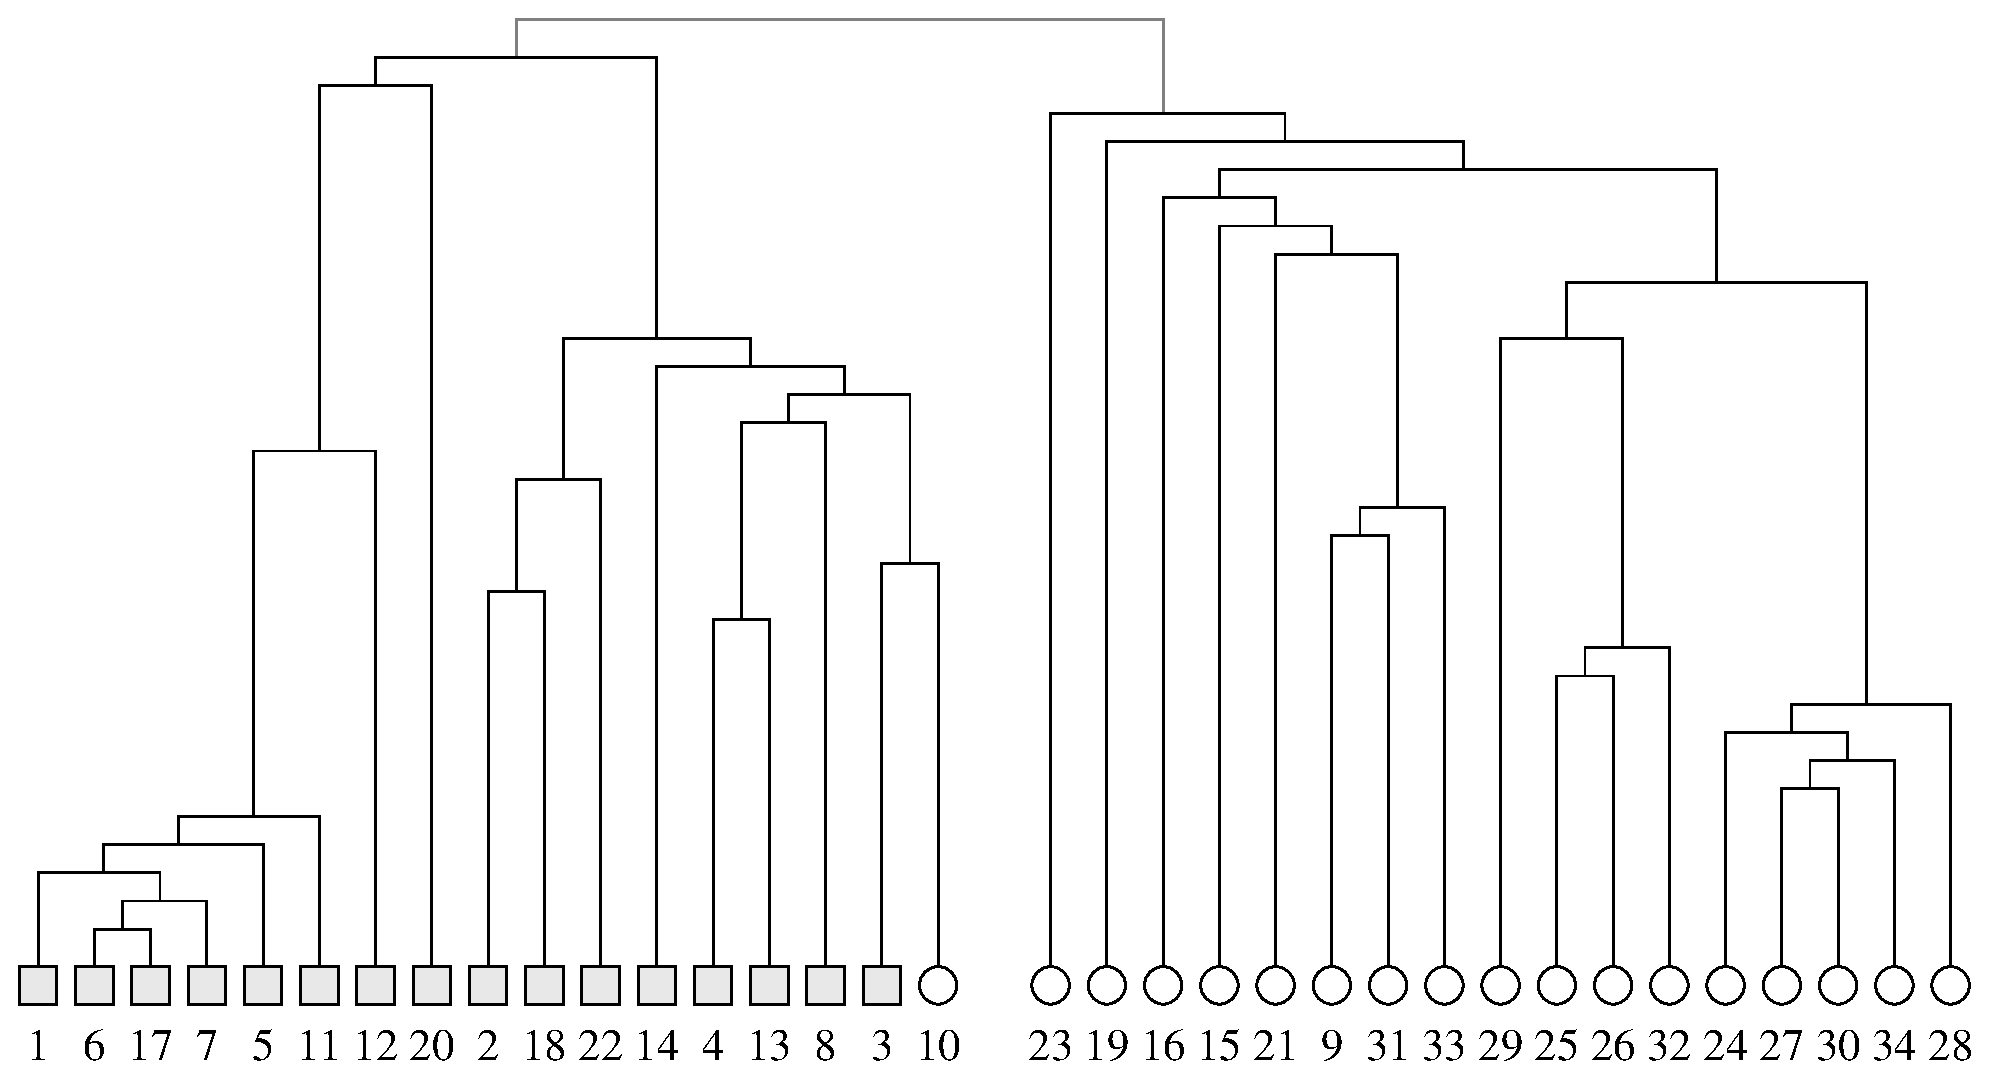
\includegraphics[width=0.7\linewidth]{0-resources/zachary}
	\caption{Dendrogram of the communities found by Newman algorithm in Zachary karate club network. This image is reprinted from \cite{Newman_greedy}.}
	\label{fig:dedro_zachary}
\end{figure}
The first modularity optimization algorithm is presented by Newman \cite{Newman_greedy},
and it is an agglomerative method. Given a graph $G(V,E)$ where $n$ are the number of nodes and $m$ the number of edges, the algorithm starts creating a supporting graph that represent the community structure. In this graph at the beginning there are all nodes and no edges between them: this represent the situation in which each node is assigned to a single cluster. The first step of the algorithm is to pick an edge from the original graph to add to the support graph such that it give the maximum increase (or minimal decrease) of the modularity with respect to the actual configuration. This value is indicated as $\Delta Q = Q_{now} - Q_{old}$ The modularity will be calculated on the full graph and not only on the "cluster" graph. Then we add the edge to the support graph: if the edges connect two sets of unconnected edges, it delivers a new partition and reducing by one the number of the partitions. So, the algorithm find $n$ different partitions of the graph (Figure \ref{fig:dedro_zachary}). 
We make some consideration of this procedure:
\begin{itemize}
\item If we add some edges that don't merge any partitions (i.e. it is internal), the modularity doesn't change.
\item Considering this, we have to calculate the modularity difference $\Delta Q$ only when we merge different partitions and so this operation is executed $n$ times.
\item Computing $Q$ requires a time of $O(m)$ that became $O(n)$ on a sparse graph.
\end{itemize}
For those reasons, the complexity of this algorithm is $O(n^2)$ on a sparse graph.
Many improvements of this algorithm were proposed later (like the Clauset et. al version \cite{Clauset_2004} that uses a max-heap to reduce the complexity to $O(n \log_2(n))$) but the complexity of the algorithm remains the biggest limit of it, even if this algorithm still allows to analyze large graphs.
\subsection{Other techniques}
The previous and Louvain algorithms are the two most famous greedy algorithms of community optimization, but other optimization strategies were proposed in the literature. A class of techniques are based on the concept of simulated annealing, i.e. an exploration of the space of the possible configuration looking for the maximum $Q$. 
Transitions between states are performed combining two types of "move": the first one assigns a vertex to a cluster chosen randomly; the second one merges or splits communities \cite{Guimer__2005}. These methods reach a very high score of modularity, near to the maximum. Unfortunately, it's very slow \cite{fortunato}. \\
To overcome this time problem, a heuristic denominated extremal optimization (EO) was proposed to perform an exploration of the space quickly. We define as fitness function $F$ of the vertex $x$ is the local modularity of $x$ divided by its degree. Starting from a random equal size bi-partitions of nodes, at each iteration a node is picked with a probability proportional to the score of the fitness measure and it is assigned to the other cluster. When there is no more improvement in modularity, the algorithm is called recursively on the two clusters. With a total complexity of $O(n^2 \log(n))$, this algorithm is a good trade-off between accuracy and speed \cite{eo}.\\ Finally, in literature it was presented the idea of combining modularity optimization with the spectral clustering. Given the adjacency matrix $A$ of the graph $G$, we define the matrix $B$ whose elements are:
\begin{equation}
B_{ij} = A_{ij} - \frac{k_ik_j}{2|V|}
\end{equation}
Modularity can be optimized by using spectral bisection on the matrix $B$ \cite{fortunato}. This algorithm has a total complexity of $O(n^2 \log(n))$.
	
	\section{Modularity Optimization}
\subsection{Sequential Algorithm}
\subsection{Parallel Algorithm}
	
	\section{Nvidia GPUs architecture and CUDA}

	
	\section{The GPU's Algorithms}
In this chapter, we present two novel parallel implementations of the Louvain algorithm: both versions implement the pruning presented by Ozaki et. al. \cite{pruning}. The first one is based on the sort-reduce pattern:
to accumulate the edges to calculate $l_{i\rightarrow C_j}$  (see formula \ref{ModularityC}),  it sorts the list and performs a reduction of consecutive values with the same key.  We also use a reduction on a sorted array to compute the maximum values of modularity for each node. 
The second algorithm uses a map to accumulate.
In this chapter, we present firstly the the algorithms, then a special speed-up technique of the first iteration of the optimization phase included in both algorithms and finally the data structure and the implementations.

\subsection{Prune-Sort-Reduce}\label{Prune-Sort-Reduce}
The Prune-Sort-Reduce Louvain algorithm is the first version of the algorithm that we present in this thesis. This algorithm implements firstly the pruning presented by Ozaki in the parallel behaviour \cite{pruning}. This algorithm uses a scheme of computation inspired by \cite{cheong2013hierarchical}: we create a list of pair $(nodes, community)$, we sort it and we aggregate the values using the node id as the key of a reduction. In the beginning, we have each node in its self-community. As the sequential Louvain algorithm, we can divide it into two steps iterated alternately: the optimization phase and the aggregation phase. 
At its turn, we divide the optimization phase in eight sub-phases, in which the operations are executed in parallel. The sub-phases from the first to sixth are executed repeatedly on some fixed part of the edges until all the edges are considered, in order to reduce the memory used simultaneously. In order to compute the right maximum values of $\Delta Q$ for each node, we split the edges into buckets such that if there is an edge with source node $n$ in the bucket, also all the other edges that belong to $n$ are included. To perform this, we use the \verb|neighbourhood_sum| vector to select the right range. We store the results at the end of the sixth sub-phases. When the algorithm compute the maximum $\Delta Q$ for each node that match the pruning criteria, we start the last two sub-phases. For the sake of simplicity, we present the case in which all edges are in exactly one bucket and all the phases are executed one after another. The phases are the following:
\begin{enumerate}
	\item \textbf{Copy sub-phase:} in the first step, we copy from the graph all the edges of the nodes that we consider in this iteration. To due this, we check on a support vector if the source nodes of the edges have a neighbour that has change community according to the criteria presented in Chapter \ref{prun}. The support vector contains boolean, it has length $n$ and in position $i$ there is a True if the nodes $i$ matched the criteria in the previous iteration, False otherwise. This vector was filled in the last phases; at the first iteration, there are only True values in it. We exclude also the self-loops because we don't consider them in the computation of the various values of $\Delta Q$. Besides, in this phase, we transform the vector of destination nodes in a vector with the associated community. Therefore, we obtain three vectors that contain the source node, the community of destination and the weight of the edges.  
	\item \textbf{Sort sub-phase:} in the second phase, we sort the vectors obtained in the first phase. We sort it using the tuple $(node, community)$ as key and the weight as value.
	To do this, we use a  \verb|thrust::zip_iterator| that allow us to consider this two vectors as if they are a unique vector of pair.  At the end of this phase, we have that all the tuples $(node, community, weight)$ with the same $(node, community)$ are consecutive. Besides, all the tuples with the same source node are consecutive.
	\item \textbf{Reduce sub-phase:} in this step we perform a reduction by key, i.e. we sum up all consecutive values with the same key. We use as key the tuple $(node, community)$: doing this, we obtain a unique tuple $(node, community,$  $tot\_weight)$ for each pair $(node, community)$. After this operation, in the weights value we have the values $l_{i\rightarrow c_j}$ related to the nodes $i$ and the community $c_j$.
	\item \textbf{Self-counting sub-phase:} In this phase, we isolate all the tuple  $(i, c, w)$ such that 
	$c$ is the actual community for the nodes $i$. We need to isolate these values because we use it in the next phase to compute the various values of $\Delta Q$.
	\item \textbf{Compute Delta sub-phase:} In this phase, given each tuple $(i, c, w)$, using the formula \ref{delta_q}, we substitute each values in the weights array with the associated $\Delta Q_{i\rightarrow c}$.
	\item \textbf{Select Max sub-phase:} Now we need to isolate the maximum $\Delta Q_{n\rightarrow c}$ for each node $n$. Considering that the vectors are already sorted, we can perform this operation using another reduction but, in this case, we return only the maximum weight instead of performing the sum. We execute this operation using the nodes vector as keys, and the other two as value, but we considering the communities only if the values $\Delta Q$ are equals. In that case, we use the minimum labelling heuristic (Chapter \ref{parallel-imp}) as braking rule.  After this step, we have exactly one tuple  $(i, c, \Delta Q_{n\rightarrow c})$  for each nodes $i$.
	\item \textbf{Update Community sub-phase:}\label{update_com} In this step, we update the community for each node if the values of $\Delta Q$ is greater than 0. We also update the related community weights: we remove the weight of the node from the previous community and we add it to the new one. These operations are atomic to avoid concurrent operations. We also implement the minimum labelling heuristic to prevent the swap of singleton nodes presented in the Chapter \ref{parallel-imp}. Besides, in this phase, we keep on a support vector of length $n$ if the nodes change communities in this iteration. This vector is different respect to the array that we use in the first step: this one store keeps track if a node change communities, the other if a node has a neighbour that change its community. In the following step, we create the second vector from the first one.
	\item \textbf{Update Pruning sub-phase:}\label{update_prun}  To update the vector that handles the pruning criteria, we firstly set all its elements to zero. After that, a method takes each edge of the graph and check if the destination edge has changed its communities in the previous iteration: if this happened, it set the corresponding node's value to True. This update operation is not atomic, because multiple threads can set only a True to the same position and there aren't conflict.
\end{enumerate}
After then we compute the new total modularity and we subtract the old value to new one: if the value is upper than a given threshold, we will repeat these steps, otherwise we start the aggregation phase. We highlight that we can not add directly the various $\Delta Q$ obtained in the optimization step to the old modularity
like the sequential algorithm, because all nodes change communities simultaneously and consequently this value is not reliable any more.\\
The aggregation phase use several similar concepts presented previously, and we can divide it into four sub-phases in which the operations are executed in parallel:
\begin{enumerate}
	\item \textbf{Re-indexing communities sub-phase:}\label{Re-indexing} in the first phase, before the graph contraction, we renumber the community. Actually, we have only certain communities associated to the nodes respect to the initial configuration: for example, if a nodes $i$ change community from $c_i$ to $c_j$ in the first iteration of the optimization phase, no nodes are assigned to $c_j$ after the update and no nodes can select the communities $c_j$ from that moment. This cause a useless waste of memory if we continue to keep all those unused values in the community weight. For this reason, we need to create a map to rearrange the communities index.
	First, we create a support vector such that at the position $c$ there is a 1 if the community $c$ has a weight greater than 0 (i.e. there is at least one node assigned to this community). Then we perform a prefix sum on this vector: in this way at the position $c$ there is the new index incremented by one for the community $c$ (please note: incremented by one because we counting from zero!). We make an example to clarify this step. We have the communities weight vector: $[0,3,0,1,0,0,4]$. We create the support vector inserting one if the weights are greater than 0 and we obtain: $[0,1,0,1,0,0,1]$. Executing the prefix sum on this vector, we obtain: $[0,1,1,2,2,2,3]$. To calculate the new index of the community $3$, for example, we have to go at the position $3$ in the vector and decrease the value by one, obtaining $1$. The values in position $0,2,4,5$, even if has a value in this vector (that in some case can be repeated), we ignore it because no nodes are in those communities, therefore we haven't index conflict. When this renumbering map is ready, we start the next phase.
	\item \textbf{Transform edges sub-phase:} In this step, all the pairs of edges $(i, j)$ of the original graph are transformed in the pair $(c_i, c_j)$ where $c_i$ is the community associated to $i$. In this phase, we also apply the map to renumber the communities that we create in the previous step. 
	\item \textbf{Sort-Reduce sub-phase:} In this phase we sort all the edges $(c_i, c_j, w)$ using as a key for the sorting the pair $(c_i, c_j)$. After this, we reduce the edges vector still using as a key $(c_i, c_j)$. After this step we have contract the graph summing up all the edges that lay between two communities.
	\item \textbf{Update variables sub-phase:}\label{updategraph}  In the last step, we update all the support value in the graph object and the community object: in particular in the first object we recalculate \verb|tot_weight_per_nodes|, \verb|neighbourhood_sum|, \verb|n_nodes| and \verb|n_links|; in the second object we assign each node to its self community and we set the communities weights consequently.
\end{enumerate}
The algorithm continues until we can not have further improvement in the modularity update. In this version of the algorithm, we keep only the best result to not occupy several device memory, but it is possible trivially save the intermediate result adding a step that copies the clustering results on the host memory after the re-indexing sub-phase (in this way we have consistent indexing among the dendrogram).
\subsection{Hashmap Version}
The second version of the parallel Louvain algorithm uses a different approach to aggregate the edges: we use a special global hashmap instead of sorted vectors.
Using a map to accumulate some values by its key is a standard approach to solve this problem because the map allows to retrieve and insert an object in $O(1)$ time. 
To obtain this performance, the hashmap uses a function named hash function to dispose at random the objects in the memory. This creates a problem on the GPU because uncoalesced memory accesses is an order of magnitude slower than sequential memory accesses. 
To overcome this problem this map uses a system of open-addressing based on the cuckoo hashing: this type of map is the one that performs better on the GPUs \cite{alcantara2012building}. This map is stored in the device global memory and uses 64 bits for the keys and 32 bits for the value. We choose to use 64 bits for the key because we need to store a pair of 32 bits keys (the pair $(node, community)$ in the optimization phase and the $(community, community)$ pair in the aggregation phase). This map has $r$ different hash function, each one associated to an id $r_i$ where $i \in [0, r-1]$. When we insert a new pair key-value $(k,v)$, we use the hash function with id $r_0$ to compute the position of the new key $v$: if the slot is empty, we add the key and the value, we use the next function $r_1$ otherwise. We continue to search a empty slot following this schema: if $r_i$ is not empty, we retry to insert the pair with function $r_{i+1}$. If all the function fails to insert the new pair, we raise an error. The main difference between this map and the classic cuckoo hashing is that we don't "kick out" the old key when we have a conflict in order to find a new memory address for it, but we hash with a different function the pair that we have to insert: this because to make a classic cuckoo hashing, we need a set of atomic operations for 128bits to do the "kick out" operation in parallel without generating race condition. This type of atomic operation in CUDA can be done only on variable up to 64 bits. Besides, this map has another special feature: if we insert a pair $(k,v)$ and there is already an entry in the table with a key $k$, the map automatically sum the values $v$ to the one stored in the map. Indeed, we use this map only to aggregate values, and for this reason, we design it to this operation as fast as possible. The last feature that we add to this table is the contract table operation: these methods re-arrange the vectors used to store the pairs in order to allow us to accessing them sequentially. After this operation, we can not get the entry using the hash function, because the memory is re-organized. We use this operation before the computation of $\Delta Q$ to increase the performance and still working considering the edges $(nodes, communities)$ independently. We describe this step later in this chapter. This contract table operation is made quickly using the function \verb|thrust::remove_if| that remove from the vector every element $x$ that satisfies a predicate and then contract the vector. The predicate that we use in this method check if the memory slot in the vector is empty. \\
Now that we have presented the map, we present the algorithm. Also, this algorithm implements the pruning operation heuristic. We can divide the optimization phase into six sub-phases.
Like the previous algorithm, we execute the first four on a fixed part of the edges to reduce the memory consumption and in these buckets, all the edges belong to a certain set of nodes, to compute the right values. When all the edges are analyzed and the results are stored, we execute the last two sub-phases. As previous, we present the case in which all edges are in exactly one bucket and all the phases are executed one after another:
\begin{enumerate}
	\item \textbf{Fill Map sub-phase:} in the first step, we fill the map with all tuple \\$(node, communities, weight)$ that has the source node that matching the criteria presented in Chapter \ref{prun}. We use the same array presented in the previous algorithm to perform this operation. We also exclude all the self-loops in this phase. At the end of this step we obtain a map where every non-empty entry has the form $(i, c_i, l_{i \rightarrow c_j})$ \ref{delta_q}. The map also isolate in a different vector each values $l_{i \rightarrow c_i}$ such that $c_i$ is the community of the nodes $i$ is stored at position $i$. This operation was made because in the delta step, after the contraction, we can not get any more the position of the entry using the hash function, and we need a method to get the nodes communities weights quickly.
	\item \textbf{Contract Table sub-phase:} in the first step, using a map to calculate $l_{i \rightarrow c_j}$ allows accessing to the memory address in $O(1)$ time for each edge. But to compute the relative delta and the maximum, we have to access the memory using an uncoalesced memory access pattern. In addition, we have no idea of how and which community are in the neighbourhood of a given node: many application allocates a thread for each edge, transform the edge destination from nodes to community and then check the maximum. This approach lay to check multiple time the score of the community $c$ if two neighbours of the nodes $n$ are in $c$. To overcome this problem, we contract the table: the vectors of the table are re-organized in order to permit sequential access, without empty slot between the entries as explained previously. After this operation, the map became a pair of vectors: at each position of the first one there is the key node-community $(i, c_j)$, in the second one the relative $l_{i \rightarrow c_j}$. The support vector with the sum of edges of the node that connects it with another in the same community is not re-arranged by this operation.
	\item \textbf{Compute Delta sub-phase:} now we can compute the $\Delta Q_{i\rightarrow c_j}$ for each tuple $(i, c_j, l_{i \rightarrow c_j})$ using the formula \ref{delta_q}. The result overwrites the last value in the tuple (we doesn't need that value any more). To get the sum of edges that connect the nodes to its actual community, we use the vector created in the first step.
	\item \textbf{Select Max sub-phase:} now we have two vector in which are stored the tuple $(i, c_j, \Delta Q_{i\rightarrow c_j})$. Now we have to select the pair $(i, \Delta Q_{i\rightarrow c_j})$ for each node $i$ such that $\Delta Q_{i\rightarrow c_j}$ is maximum. We can not use as the previous algorithm a reduce operation because we haven't a sorted array and the sorting operation is too expansive. Instead, we declare two support array of length $n$ where $n$ is the number of nodes. Then, for each tuple, we use the \verb|atomicMax| operation to check if the value $\Delta Q_{i\rightarrow c_j}$ is greater than the one saved in the first support array at the position $i$: if it is, we substitute the value in the first one with $\Delta Q_{i\rightarrow c_j}$ and the value in the second one with $c_j$, we don't do anything otherwise. To avoid race condition caused by the two atomic operation (\verb|atomicMax| on the value and eventually \verb|atomicCAS| for the associated community), in the implementation we transform the pair $(c,\Delta Q_{n\rightarrow c})$ of 32 bits variable in a unique word of 64 bit. The half most significant bytes are filled by the value, the other part by the community. Thanks to this, we can use an unique \verb|atomicMax| to substitute both the values. At the end of this step, we have exactly one tuple  $(i, c, \Delta Q_{n\rightarrow c})$ for each node $i$, like the previous algorithm. Now we can update the communities and the pruning support vector similar the other version above.
	\item \textbf{Update Community sub-phase:} This phase update the community just like the one presented in the Prune-Sort-Reduce version (\ref{Prune-Sort-Reduce}, optimization sub-phase \ref{update_com}).
	\item \textbf{Update Pruning sub-phase:} This phase create the array with the pruning information just like the one presented in the Prune-Sort-Reduce version (\ref{Prune-Sort-Reduce}, optimization sub-phase \ref{update_prun}).
\end{enumerate}
We continue to execute this step until the difference in modularity between the configuration drops below a given threshold. The consideration of the computing of $\Delta Q$ in parallel behaviour presented in the previous chapter is still valid. \\
The aggregation phase of this algorithm use once again the map to aggregate, but the key in this context is composed of $(community_source, community_destination)$. We can divide this phase in four sub-phase like the previous version:
\begin{enumerate}
	\item \textbf{Re-indexing communities sub-phase:} This phase created the map that allows the re-indexing of the communities as the one presented in the Prune-Sort-Reduce version (\ref{Prune-Sort-Reduce}, aggregation sub-phase \ref{Re-indexing}).
	\item \textbf{Communities map sub-phase:} In this step, all the tuple of edges $(i, j, w)$ of the original graph are inserted in a hash table. Before the insertion, we transform each entry in the tuple $(r_i, r_j, w)$ where $r_i$ is an index of the community associated with $i$ after the remapping. We use as key the pair $(r_i, r_j)$. At the end of this step, we have each edge of the new graph, because we sum up all the edges that lay between two communities.
	\item \textbf{Contract-sort sub-phase:} At the beginning of this phase, we have a map containing all the edges of the new graph. However, the graph object store the edges information using three ordered vectors, so we have to re-organize the information stored in the unordered and uncoalesced map. To do this, we use the contract operation to transform the map in two vector $(key, value)$ and then we sort the arrays according to the order of the first one. Finally, we update the graph: during this operation, we split the unique composite key in the pair $(source, destination)$ and we copy the value in the relative vector in the graph object. We copy the weight vector without performing an additional operation. 
	\item \textbf{Update variables sub-phase:} This phase update the new graph and the related communities object just like the one presented in the Prune-Sort-Reduce version (\ref{Prune-Sort-Reduce}, aggregation sub-phase \ref{updategraph}).
\end{enumerate}
Like the previous algorithm, this one continues to alternate the two main phases until no further improvement in the modularity update can be obtained.
\subsection{Speed-up the First Iteration in the Optimization Phase}\label{f-1}
In this chapter, we present an optimization technique that we add into our code to speed-up the first iteration of each optimization phase. We include this method in both versions of the algorithm presented previously. We focus this presentation on the Prune-Sort-Reduce version, even if the concept that allows us to optimize the algorithm is still present in the Hashmap version. At the beginning and also after each aggregation phase, we notice that we have a configuration in which each node is assigned to each self-community, i.e. each node $i$ is assigned to the community $i$ and it is the only node assigned to it. In this configuration, when in the copy sub-phase we transform each edge $(i,j)$ in the pair $(i,c_j)$ where $c_j$ is the community of the node $j$, we obtain the same original pair, because the index of $c_j$ is equal to $j$. In addition, considering that each node is assigned to a different community, we don't need the sort and reduce sub-phases, because the pairs $(i, j)$ are already sorted by the construction of the graph object (n.b. we need a sorted vector for the select max sub-phase) and the reduction is useless, because all the pairs have a different composite key $(i, j)$.
Also the self-counting sub-phase is useless, because no edge that isn't a self-loop lay a node in the same community and during the copy sub-phase we excluding the self-loop from the computation. 
Considering all these facts, we choose to remove in the first iteration this three sub-phases and also to avoid the useless transformation in the copy sub-phase. For the Hashmap version of the algorithm, we still use this optimization based on the other version because we use the hashmap to aggregate different edges and this aggregation is no longer necessary.

\subsection{Data Structures}
The two main structures that we need to represent are the original graph and the community structure. Commonly a graph $G(V, E)$ is represented using its adjacency matrix: each node is associated with an incremental id in the range $(0, n-1)$ where $n$ is the number of nodes. To retrieve the weights of an edge between two nodes, we look to the values stored at the position $(id_1, id_2)$. As we say in the chapter \ref{3.1}, the community detection techniques are executed on sparse graph to make sense.  Therefore, if we use a matrix to represent a sparse graph, this matrix will have a lot of zeros and only some values different from it. Even if this pattern allows to retrieve the weight of an edge in constant time, this data structure isn't suitable for a problem that involves millions of data because we need too much memory to allocate this matrix that has several unused values. Therefore we have the necessity of compress the adjacency matrix. To do this, we choose to represent it using a coordinate list (often referred to as COO). We have three vectors \verb|edges_source|,  \verb|edges_destination| and  \verb|weights| that contain respectively the ids of the rows, the ids of the columns and the values. The standard modularity optimization is computed on undirected graphs: this means that the adjacency matrix is symmetric and we can store in the COO list only the upper triangle of the matrix and we still have all the edges represented. Despite this observation, we store all the values of the adjacency matrix because we need those repeated values in these algorithms. In fact, we consider the values in the first array as the source node of the edges and the values in the second one as the destination node of the edges. As we describe in the following section, we transform the vector that contains the destination nodes to a vector that contains the destination community. To have always all edges even in this new behaviour, we have to represent every edge twice in this structure reverting the order of the source and the destination. These vectors are also sorted by the pair $(source, destination)$ and there is a vector named  \verb|neighboorhood_sum| of length $n$ in which at position $i$ there is the starting position of the edges that have source $i$ in \verb|edge_source|. Thanks to this vector, we can retrieve fast all the neighbour of a given node. These particular COO lists are also known as compressed neighbour lists. In the graph object, we also store a vector named \verb| tot_weight_per_nodes| that associate each node $i$ to its degree, the total degree of the graph, the number of nodes and the number of the edges. We use \verb|thrust::device_vector| to store all this data on the GPUs memory. In summary, the graph object is the following:\\
\begin{lstlisting}[language=C++]
struct GraphDevice {
unsigned int n_nodes;
unsigned long n_links;
double total_weight;

thrust::device_vector<unsigned> tot_weight_per_nodes;
thrust::device_vector<unsigned int> neighbourhood_sum;

thrust::device_vector<unsigned int> edge_source;
thrust::device_vector<unsigned int> edge_destination;
thrust::device_vector<unsigned int> weights;
}
\end{lstlisting}
To represent the communities, we use another object that contains the graph associated with it. We notice that the maximum number of different communities is pair to the total number of nodes: this is also the configuration at the beginning of the algorithm.  Considering this, we choose to identify each community with an incremental id in the range $(0, n-1)$, like we do previously with the nodes. Therefore, in the community object, we have a vector named \verb|communities| of length $n$ in which in the position $i$ there is the id of the community of the node $i$. Besides, there is a vector of size $n$ that associate each community to its total weight.  In summary,  the community object is the following:\\
\begin{lstlisting}[language=C++]
struct Community {
GraphDevice graph;

thrust::device_vector<unsigned int> communities;
thrust::device_vector<double> communities_weight;
}
\end{lstlisting}
	
	\section{Performance and Analysis}\label{C6}
In this chapter, we present the results obtained by these two algorithms. We use 13 datasets to test the algorithms, and we analyze the performances globally on the entire algorithm but also locally on specific phases and sub-phases to highlight the point of strengths and the weakness of both algorithms. In this chapter, we firstly present the datasets on which we have executed our test. Then we give an overlook of the results obtained. They are useful for the subsequent analysis which, in turn, we dived in two parts: in the first part we analyze the contribution of the pruning approach on each algorithm; in the second part we make a comparison between the two algorithms, to enhance when one algorithm performs better than the other. These considerations are on base to the adaptive algorithm that we present in the next chapter. It implements the logic of the two algorithms and selects to use the best based on the situation, so the information that we have collects in this part are fundamental for the design choice that we make. 

\subsection{Datasets}\label{Dataset}
In this section, we present the 13 datasets used in this thesis. These datasets coming from three main sources: the Stanford Stanford Large Network Dataset Collection (also known as SNAP) \cite{snap}, the Florida Sparse Matrix Collection \cite{florida-matrix} and the Koblenz Network Collection (also known as KONECT)  \cite{konect}. In Table \ref{tab:dataset} there is a brief presentation of the dataset and in Figure \ref{fig:dataset-degree-distribution} there is the degree distribution of the graphs.  We point out that even if all this graph is unweighted, some of it is directed: during the parsing phase we doesn't keep the "directness" of the graph, and we treat it as an undirected one as required from the algorithm. In addition, if in the original graph there are some repeated edges, we consider it once. In the table \ref{tab:dataset} the number of edges is those obtained after this parsing, ordered by increasing edges number. Now we present the datasets: 
\begin{table}
	\centering
	\begin{tabular}{ |l||c||r|r|}
		\hline
		\multicolumn{4}{|c|}{Datasets} \\
		\hline
		Name& Source &  Number of nodes  & Number of edges\\
		\hline
		coPapersDBLP & Florida  & 540 486    & 15 245 729\\
		patentCite & KONECT &3 774 768 & 16 518 947 \\
		packing-500x100x100-b050 & Florida & 2 145 839 & 17 488 243 \\
		soc-pokec-relationship & SNAP &1 632 803 & 22 301 964 \\ 
		delaunay\_n23 & Florida &8 388 608 & 25 165 784\\
		soc-LiveJournal1 & SNAP & 4 847 571 & 43 369 619 \\
		wikipedia\_link\_ja & KONECT & 1 610 638 & 56 237 763\\
		hollywood-2009 & Florida &1 139 905 & 57 515 616 \\
		wikipedia\_link\_it & KONECT & 1 865 965 & 68 049 979\\
		wikipedia\_link\_fr & KONECT & 3 023 165 & 83 472 152\\
		com-orkut & SNAP &3 072 441 &117 185 083\\
		wikipedia\_en(dbpedia) & KONECT & 18 268 991 & 126 890 209 \\
		indochina-2004 & Florida & 7 414 768 & 153 487 303 \\
		\hline
	\end{tabular}
	\caption{\label{tab:dataset}Datasets overview}
\end{table} 
\begin{itemize}
	\item \textbf{coPapersDBLP:} this graph model the citation and co-author network from the DBLP - Digital Bibliography and Library Project. Each node represents an author and each edge a citation.
	\item \textbf{patentCite:} This is the citation network of patents registered with the United States Patent and Trademark Office. Each node is a patent, and a directed edge represents a patent and an edge represents a citation. The network contains loops. This graph is also directed.
	\item \textbf{packing-500x100x100-b050:} this is a synthetic graph from numerical simulation.  
	\item \textbf{soc-pokec:} Pokec is the most popular online social network in Slovakia. Pokec has been provided for more than 10 years and connects more than 1.6 million people. This dataset map the relationship between people.
	\item \textbf{delaunay\_n23:} given a random set of point, in this graph represent a Delaunay triangulations of them.
	\item \textbf{soc-LiveJournal1}: LiveJournal is a free online community with almost 10 million members; a significant fraction of these members is highly active. LiveJournal allows members to maintain journals, individual and group blogs, and it allows people to declare which other members are their friends they belong. This graph model these friendship relations. 
	\item \textbf{wikipedia\_link\_jp:} This network consists of the wikilinks of Wikipedia in the Japanese language (.ja). Nodes are Wikipedia articles, and directed edges are hyperlinks. Only pages in the article namespace are included. This graph is directed and some self-loop is possible.
	\item \textbf{hollywood-2009}: The graph of           
	movie actors. Vertices are actors, and two actors are joined by an edge whenever they appeared in a movie together. The data date back to 2009. 
	\item \textbf{wikipedia\_link\_it:} This network consists of the wikilinks of the Wikipedia in the Italian language (it). Nodes are Wikipedia articles, and directed edges are hyperlinks. Only pages in the article namespace are included. This graph is directed and some self-loop is possible.
	\item \textbf{wikipedia\_link\_fr:} This network consists of the wikilinks of Wikipedia in the French language (.fr). Nodes are Wikipedia articles, and directed edges are hyperlinks. Only pages in the article namespace are included. This graph is directed and some self-loop is possible.
	\item \textbf{com-orkut:} Orkut is a social network where users form a friendship with each other: the nodes represent the users and the edges the friendship between them.
	\item \textbf{wikipedia\_en (dbpedia)}: The network is the hyperlink network of Wikipedia, as extracted in DBpedia. Nodes are pages in Wikipedia and edges correspond to hyperlinks (also known as wikilinks). The edges correspond to the relationships in DBpedia.
	Network info. The original graph is directed and multiple edges are possible.
	\item \textbf{indochina-2004}: A fairly large crawl of the country domains of Indochina performed for the Nagaoka University of Technology. This is a directed graph and each node represent a site and each edge a link from one site to another.
\end{itemize}

\begin{figure}
	\centering
	\includegraphics[width=1\linewidth]{0-resources/dataset-degree-distribution.png}
	\caption{Degree distribution in the datasets: we divide the nodes into ordered classes wherein the class $i$ there are all the nodes with a degree in the range $[2^i, 2^{i+1})$. On the $x$-axes there are these classes; on the $y$ axes there is the percentage of nodes assigned to them.}
	\label{fig:dataset-degree-distribution}
\end{figure}
\newpage
\subsection{Results Overview}
In this section, we present an overview of the obtained results and we make some general consideration about it. Some more insights about the first optimization phase and about the aggregation phase are presented next and we make some consideration in light of what we present in this section.\\ 
The algorithms were run on a Ubuntu 18.04.4 LTS machine with a 2.10GHz  Intel(R) Xeon(R) Silver 4110 CPU, a TITAN Xp GPU with 12 GB of memory and CUDA 10.2. To run our code we need an Nvidia GPU with a compute capability $\geq$ 3.5 due to the 64 bits \verb|atomicMax| operation used in PH-Louvain. This GPU has a compute capability 6.1, so it complies with the technical specification.
We remark that we keep executing our optimization phase until the value of $\Delta Q$ between the various iteration is greater than a threshold $t$. Both our parallel version in the test uses $t = 0.01$.\\
\begin{table}[h]
	\centering
	\begin{tabular}{ |l||r||r|r|}
		\hline
		\multicolumn{4}{|c|}{Modularity Score} \\
		\hline
		Graph & Sequential & PSR-Louvain & PH-Louvain \\
		\hline
		coPapersDBLP 			& 0.8490 & 0.8544 & 0.8544 \\
		patentCite 				& 0.8095 & 0.7911 & 0.7878 \\
		packing-500x100x100-b050& 0.9353 & 0.9434 & 0.9416 \\
		soc-pokec-relationship	& 0.6837 & 0.6934 & 0.6852 \\ 
		delaunay\_n23 			& 0.9881 & 0.9856 & 0.9857 \\
		soc-LiveJournal1 		& 0.7251 & 0.7491 & 0.7482 \\
		wikipedia\_link\_ja 	& 0.5928 & 0.5690 & 0.5724 \\
		hollywood-2009 			& 0.7511 & 0.7542 & 0.7542 \\
		wikipedia\_link\_it 	& 0.7221 & 0.7190 & 0.7196 \\
		wikipedia\_link\_fr 	& 0.6777 & 0.6834 & 0.6871 \\
		com-orkut 				& 0.6545 & 0.6613 & 0.6629 \\
		wikipedia\_en(dbpedia) 	& 0.6629 & 0.6612 & 0.6618 \\
		indochina-2004 			& 0.9638 & 0.9632 & 0.9632 \\
		\hline
	\end{tabular}
	\caption{\label{tab:mod}Modularity result}
\end{table} \\
First of all, we analyze the modularity score obtained by the two algorithms respect to the sequential version as presented in \cite{Blondel_2008} to check the correctness of our algorithms. In Table \ref{tab:mod}, the obtained results are presented. We notice that both the score of the algorithm are in pair between them and also with the sequential version for all the graphs, and in some case, we obtain also a better result in the parallel implementations respect to the sequential version. This may be due to the parallel optimization, changing all the communities assigned to the vertices simultaneously, can avoid some local maxima.
\begin{table}
	\centering
	\begin{tabular}{ |l||r||r|r|}
		\hline
		\multicolumn{4}{|c|}{Execution Times} \\
		\hline
		Graph & Sequential & PSR-Louvain & PH-Louvain \\
		\hline
		coPapersDBLP 			&  11 906.89 &   419.59 &  412.79 \\
		patentCite 				&  88 620.13 & 1 796.88 & 2 555.14 \\
		packing-500x100x100-b050&  13 746.14 & 1 045.25 & 1 090.03 \\
		soc-pokec-relationship	&  30 162.70 & 1 843.95 & 2 186.81 \\ 
		delaunay\_n23 			&  44 392.42 & 1 020.23 & 1 319.22 \\
		soc-LiveJournal1 		&  77 225.64 & 2 187.45 & 2 677.51 \\
		wikipedia\_link\_ja 	&  76 816.01 & 2 654.88 & 2 305.11 \\
		hollywood-2009 			&  52 306.71 & 2 092.09 & 1 758.27 \\
		wikipedia\_link\_it 	&  82 599.92 & 3 875.04 & 2 732.99 \\
		wikipedia\_link\_fr 	& 115 977.81 & 3 910.95 & 3 273.91 \\
		com-orkut 				& 193 835.34 & 7 566.90 & 7 484.10 \\
		wikipedia\_en(dbpedia) 	& 300 431.38 & 5 287.65 & 6 464.03 \\
		indochina-2004 			& 113 195.87 & 2 899.50 & 2 303.52 \\
		\hline
	\end{tabular}
	\caption{\label{tab:execution_time}Execution Time in milliseconds}
\end{table} \\
In Table \ref{tab:execution_time}, there are the execution times of the two algorithms respect to the sequential version. We notice a big improvement in the performance for both the algorithm respect to the sequential version: we obtain a speed-up in range of a variable factor from 12 to 56 for our two algorithms. 
Besides, we notice that, according to the graph analyzed, the two algorithms obtain different performance. In some case, one approach outperforms the other of even more than one second. In the following sections, we analyze in details these two algorithms to discover the motivation of these different performances.  
\subsection{Pruning analysis}
In this section, we analyze the effectiveness of the pruning approach: we focus our research on the first optimization phase. As we said previously, the first optimization phase is the most time-requiring, consuming about 80\% of the time \cite{wickramaarachchi2014fast}, so the pruning approach should increase the performance especially in this phase. For this reason, we concentrate our analysis of this technique over it.
\begin{figure}[h]
	\centering
	\includegraphics[width=1\linewidth]{0-resources/edge-percentage}
	\caption{Percentage of edge analyzed in the first optimization phase.}
	\label{fig:edge-percentage}
\end{figure}
First of all, we present the percentage of the edges that we analyze in each iteration of the optimization phase (Figure \ref{fig:edge-percentage}). The number of the edges analyze are quite similar for both the algorithms. Excluding certain fluctuation at the earliest stage (we remark also that the two graph with the highest noise is two synthetic ones, i.e. packing-500x100x100-b050 and delaunay\_n23), we notice that the portion of the edges analyzed tend to decrease iteration by iteration. The percentage of reduction highly depends on the graph examined: we have the smallest reduction for the wikipedia\_link\_ja (only the $\sim\%2$ of the total are excluded in the last iteration); instead, in the graph packing-500x100x100-b050, we have run the optimization only on the $\sim\%50$ of the graph edges in the last iteration. Our study on the dataset doesn't find any direct correlation between the decrease of the number of the edges analyzed and the degree distribution of the nodes, presented in Figure \ref{fig:dataset-degree-distribution}.
\subsubsection{PSR-Louvain analysis}
\begin{figure}[h]
	\centering
	\includegraphics[width=1\linewidth]{0-resources/sort-prune-vs-no-prune}
	\caption{Comparison of the execution time between the Prune-Sort-Reduce (in blue) and a version of comparison without the Pruning approach (in orange) for each execution of the first optimization phase, excluding the first one.}
	\label{fig:prun-vs-no}
\end{figure}
\noindent Now we evaluate the impact in terms of times of the pruning approach in the PSR-Louvain algorithm: to do this, we create a comparison version of the algorithm from the presented one. This version doesn't prune the node in the Copy sub-phase and doesn't collect the data used to create the support pruning array in the last two sub-phases (the first one only update the community assign to each node; the second one is skipped). The execution times of each iteration of the first phase are illustrated in Figure \ref{fig:prun-vs-no}. We exclude from this graphic the first iteration because this one doesn't make the same step of the other due to its special optimization (Chapter \ref{f-1}). We notice that the reduction in terms of times in the pruning version is proportional to the reduction of edges analyzed: in the graph in which the reduction of the edges analyzed highly decrease, the pruning version outperforms the standard version; in the graph in which the reduction in terms of edges are small, the execution times are quite similar: the pruning algorithm is slower up to $\sim15$ ms at iteration (in dbpedia-link) because the computation of the pruning information requires some extra time but the reduction that leads to is smaller. In general, we see that the ratio between execution times of the pruning version and the non-pruning one is in pair with the number of nodes pruned in each iteration. We notice also that the execution times decrease iteration by iteration even for the version without the pruning: this is caused by the reduction in terms of the time of the delta computation sub-phase, as we can see in the \ref{fig:livejournal-comparison} is illustrated the contribution of each sub-phase in terms of time to for each iteration for the pruning version and the standard in the LiveJournal1 dataset.
\begin{figure}
	\centering
	\includegraphics[width=1\linewidth]{0-resources/livejournal-comparison-sort.png}
	\caption{Comparison of the execution time between the Prune-Sort-Reduce (on the left) and a version of comparison without the Pruning approach (on the pruning) for each execution of the first iteration phase in the LiveJournal1 dataset. We highlight the contribution of each sub-phase in terms of time.}
	\label{fig:livejournal-comparison}
\end{figure}
We notice that the Sort sub-phase is the most consuming one and this behaviour is similar also in the other graph: this sub-phase at least 50\% of the time, reaching a peak of even more than 80\% of the time in the first and the last graph (Figure \ref{fig:suphases-sort}). From the Figure \ref{fig:livejournal-comparison}, we notice also that the pruning on the data in the input has a direct effect on the sorting phase and the decreasing in terms of time is proportional to the number of the edges pruned (as we can see by comparing Figure \ref{fig:suphases-sort} and Figure \ref{fig:edge-percentage}). The pruning update sub-phase has a small impact on the total execution time. 
\begin{figure}[t!]
	\centering
	\includegraphics[width=1\linewidth]{0-resources/suphases-sort}
	\caption{Contribution of each sub-phase in terms of time for each iteration of the first optimization phase. }
	\label{fig:suphases-sort}
\end{figure}
In conclusion, even if the pruning approach isn't always effective and can introduce a little overhead, the gain in terms of time that we obtain when we prune a portion of the edges are high, therefore adding the pruning approach is a valid optimization technique for the algorithm that uses a sort-reduce pattern to aggregate. 
\subsubsection{Hashmap algorithm analysis}\label{hashmap-analysis}
\begin{figure}[h]
	\centering
	\includegraphics[width=1\linewidth]{0-resources/hash-prune-vs-no-prune}
	\caption{Comparison of the execution time between the Hashmap (in blue) and a version of comparison without the pruning approach (in orange) for each execution of the first optimization phase, excluding the first one. }
	\label{fig:hash-prune-vs-no-prune}
\end{figure}
\noindent We evaluate the impact in terms of time of the pruning approach in the PH-Louvain algorithm as before: we compare the algorithm with another test version in which we have removed the pruning. In Figure \ref{fig:hash-prune-vs-no-prune} there are the execution times of the first optimization phase for each iteration of both two versions. As previous, we exclude from this graphic the first iteration. \\
We notice that the two algorithms perform generally in a similar way, with a significant difference only when the pruning reduce considerably the number of edges: the pruning algorithm is slower up to $\sim25$ ms at iteration (in the graph dbpedia-link), caused by the extra time to compute the pruning information. Even if we reduce the execution time reducing the number of edges analyzed, the gap between the two version is not directly proportional to the number of edges pruned like in the previous version: this is due to the branching problem for thread in the same warp. \\
During the Fill Map sub-phase, we insert in the map each pair node-community such that the nodes have almost one neighbour that change community in the previous iteration.
To perform this operation, an edge $(source, destination)$ is assigned to each thread: than it checks if the source node matches the pruning requirement, it changes the destination node with the destination communities and inserts the value in the map. If an edge has a source node that doesn't match the criteria, its thread will return without doing nothing else. The problem is that the nodes are organized in a warp of 32 threads assigned to a core of the Streaming Multiprocessor: the GPU execute a new warp on the same core only when all thread of the old warp finish the execution. If in a warp there is even just one thread that has to insert the pair in the map, all the other thread have to wait for it. This reduces the gain in terms of times in the Fill-Map sub-phase.
\begin{figure}[t!]
	\centering
	\includegraphics[width=1\linewidth]{0-resources/suphases-hash}
	\caption{}
	\label{fig:suphases-hash}
\end{figure}

We notice that in the no-pruning version the execution time tend to strongly decrease even in the case in which the pruning doesn't remove a considerable part of the edges (like the wikipedia\_link\_jp dataset), so we analyze the sub-phases to see what change between each iteration: in the Figure \ref{fig:suphases-hash} is illustrated the consuming time of each sub-phase compared to the total time of each iteration.
The most consuming sub-phase is the fill map one:  this sub-phase at least 50\% of the time, reaching a peak of even more than 75\%. We notice that at each iteration, the times required decrease: therefore we focus our analysis on this behaviour of the map. We analyze the number of conflicts that we have when we try to insert a new key in the map. 
We notice that the number of conflicts in the map decrease iteration by iteration: the reason is that, at each iteration, the number of different keys inserted decrease. Indeed, at every iteration the number of communities decrease because similar nodes tend to converge to one community for groups: this reduces the number of possible different keys node-community that we have. 
Then, we analyze the number of different keys inserted in the map at each iteration.\\
\begin{figure}[t!]
	\centering
	\includegraphics[width=0.7\linewidth]{0-resources/time-vs-possible-keys}
	\caption{Execution time of the Hashmap version in relation to the number of different pair (node, community) inserted (expressed with respect to the maximum number of keys).}
	\label{fig:time-vs-possible-keys}
\end{figure}
\noindent In Figure \ref{fig:time-vs-possible-keys}, we have on the x-axis the number of different keys at that iteration in relation to the maximum possible number of keys (i.e. the number of edges, because we have the maximum when each node is in its self-community); on the y-axes we have the execution times. We notice that there is a direct correlation between this data and this two values, and this explains why the PH-Louvain algorithm performs better in the last iterations with respect to the first ones. 
\newpage
\subsection{Algorithms comparison}\label{alg-comp}
\begin{figure}[h]
	\centering
	\includegraphics[width=1\linewidth]{0-resources/modularity-progression}
	\caption{Modularity Progression in the first ten iteration of the optimization phase.}
	\label{fig:modularity-progression}
\end{figure} 
\noindent In this section, we focus our analysis on the comparison between the two algorithms in order to find the advantages and disadvantages of each method. 
First of all, we notice from Table \ref{tab:mod} that the two algorithms obtain a very similar score of modularity. In Figure \ref{fig:modularity-progression}, we expose the progression of the modularity $Q$ in the first operation. As we can see, the modularity in the two algorithms grows in an almost identical way: this is due to the minimum labelling heuristic (Chapter \ref{parallel-imp}) that force the algorithms to converge to a similar result. \\
\begin{figure}[t!]
	\centering
	\includegraphics[width=1\linewidth]{0-resources/first-hash-sort}
	\caption{Comparison of the execution time of the first iteration of the first optimization phase between the two presented versions unoptimized of the algorithm and the optimized version.}
	\label{fig:first-hash-sort}
\end{figure}
To analyze the differences in terms of performance, we start analyzing the impact of the optimization of the first iteration of the optimization phase for both the algorithms. We are expecting a huge reduction in terms of times, considering that we remove the most consuming time phase from the Prune-Sort-Reduce routine, i.e. the sorting phase. As shown in the Figure \ref{fig:first-hash-sort}, we obtain the expected results: we obtain a reduction in a range between $\sim 51\%$ and $\sim 86\%$ respect to the PSR-Louvain not optimized and a reduction in a range between $\sim 84\%$ and $\sim 95\%$ respect to the PH-Louvain not optimized. From the data we also see that in the second algorithm, this optimization introduce a little delay in the next iteration respect to the first one: this is caused by the deallocation of the support variable used in the fast approach (that are the same used in the PSR-Louvain) and the allocation of the hashmap and other support variables. But, this overhead is much smaller than the gain obtained by the optimization, therefore we consider it a valid technique to improve the performance.\\
From Figure \ref{fig:first-hash-sort}, we also note that the PH-Louvain is always slower with respect to the PSR-Louvain, and for this reason, this technique has a greater impact on it. Considering this particular feature, we choose to go further in our analysis: we compare the iterations of the first optimization phase in terms of times of the two version of the algorithms, excluding the first iteration.
\begin{figure}[t!]
	\centering
	\includegraphics[width=1\linewidth]{0-resources/hash-vs-sort}
	\caption{Execution time in the first ten iteration of the first optimization phase, excluding the first optimized iteration.}
	\label{fig:hash-vs-sort}
\end{figure}
In Figure \ref{fig:hash-vs-sort} are exposed the results. We notice that the second iteration of the PH-Louvain is always slower respect to the PSR-Louvain.
Considering the observation presented in the previous chapter, we conclude that in the first iterations the PH-Louvain algorithm suffers respect to the other due to the high number of different pair key-community that we insert in the map. 
On the other hand, if the number of different pair drops below a given value, the hashmap performs better.
Instead, the PSR-Louvain does not benefit from a similar behaviour and its performances are generally more stable (they are improved consistently only by the pruning). 
We analyze similarly also the other optimization phases (Figure \ref{fig:multi-phase:optimization}). 
We notice that, from the second optimization phase, generally the PSR-Louvain performs better in terms of total time (i.e. the sum of the times of each iteration) than the PH-Louvain: this because the number of iteration generally decrease phase by phase and the first approach generally performs better than the second one in the first iterations of the phase. Even if the number of conflicts decreases (since we allocate in a map with the same order of magnitude of the first phase in the following phases), also the time of the sorting sub-phase of the other algorithm decrease: to see an improvement of the hashmap respect to the other approach we need a convergence similar to the one saw in the first optimization phase.
For these reasons, the sorting version of the algorithm tends to perform better than the hashmap one from the second optimization phase. \\
We study also the difference between the algorithms in terms of aggregation phases: the results of our study are presented in Figure \ref{fig:multi-phase:aggregation}.
We notice that the execution times of the PH-Louvain tend to perform better with respect to the PSR-Louvain. Considering the observation about the performance of the hashmap that we made previously, it is easy to motivate these performance results. The hashmap performs better respect to the sorting approach when the number of keys decreases consistently. In the aggregation phase, the number of active communities is decreased compared to the starting situation. Besides, in this phase we insert in the map a key composed by the two communities id: this involves a further reduction of the number of keys inserted because we tend to insert more often the same key in the map. Therefore the performance is related to the number of different active communities find at the end of the optimization phase: indeed the only two cases in which the sort-reduce version perform better than the hashmap version are those in which the number of communities is decreased slightly in relation to the number of edges (i.e. the maximum possible number of communities).
All of these considerations are at the base of the design of an adaptive approach that we present in the next section: indeed, we can estimate if the PH-Louvain performs better then the other algorithm by the comparing of the number of different keys in relation to the number of the possible one, and select the right algorithm to use.	
\begin{figure}[t!]
	\hspace*{-4em}
	\subcaptionbox{\label{fig:multi-phase:optimization}}{\includegraphics[width=0.6\linewidth]{0-resources/optimization-phases.png}}
	\hspace{2em}%
	\subcaptionbox{\label{fig:multi-phase:aggregation}}{\includegraphics[width=0.6\linewidth]{0-resources/aggregation-phase.png}}
	\caption{(a): Execution times of the first four optimization phases;\\(b) Execution times of the first four aggregation phases.}
\end{figure}
\newpage
\section{Adaptive Louvain Algorithm}\label{C7}
In this chapter, we finally present the adaptive algorithm: it uses a heuristic to switch from the sort-reduce version to the hashmap version when the number of different node-community keys falls below a certain threshold. This threshold is calculated in percentage with respect to the total number of possible keys, i.e. the number of edges. Next, we analyze the result of this new algorithm, comparing it to the two original algorithms that we presented previously and other two implementation of the Louvain heuristic, integrated in two important libraries for the graph analysis on the GPU: cuGraph \cite{cuGraph} and Gunrock \cite{gunrock}. 
\subsection{Algorithm}
Our adaptive Louvain algorithm for the GPU combines the Prune-Sort-Reduce algorithm and the Hashmap algorithm in order to select the best behaviour basing the choice on the situation. \\ In the previous chapter, we showed that the Prune-Sort-Reduce algorithm performs better than the Hashmap in the first iteration of the optimization phase. We also showed that, if the number of different key falls below a given threshold, the Hashmap version starts to perform better than the Prune-Sort-Reduce version.\\
Based on these considerations, we design the optimization phase of our adaptive algorithm as following, bearing in mind that we keep iterating this phase until the difference of modularity $\Delta Q$ between the iteration is greater than a given threshold  $T_{\Delta Q}$:
\begin{enumerate}
	\item At the beginning, we optimize the first iteration of the optimization phase using the optimized approach presented in Chapter \ref{f-1}.
	\item Next, in the second iteration, we use the Prune-Sort-Reduce version of the optimization phase, with one addition compared to the standard version: we keep track of the number $k^*$ of different tuples $(i,c_j,l_{i\rightarrow c_j)}$ that we have after the Reduce sub-phase,  where $i$ is the source node, $c_j$ is the destination community and $l_{i\rightarrow c_j}$ is the sum of all the edges that link the node $i$ with a node in the community $c_j$ . This value is the number of different keys that we would insert in the map if we had used the other version of the optimization phase.
	\item From the third iteration onwards, before anything else, we divide the value of $k^*$ by the total number of edges $m$: the second value is equal to the maximum number of different keys that we can insert in the hashmap, i.e. the situation that each node is in each own community. If the value $\frac{k^*}{m}$ falls below a given threshold $T_{key}$, we execute the following iteration using the Hashmap approach, otherwise, we use the Prune-Sort-Reduce one. 
\end{enumerate}
\begin{figure}[t!]
	\centering
	\includegraphics[width=0.7\linewidth]{0-resources/adaptive_schema}
	\caption{Schema of the Adaptive Optimization phase: before starting a new optimization routine, we check if the value $\frac{k^*}{m}$ falls below a given threshold: if it happens, we will use the hashmap based routine, otherwise we use the sort-reduce routine.}
	\label{fig:adaptiveschema}
\end{figure}
Figure \ref{fig:adaptiveschema} shows a schematic diagram of the optimization phase. It is technically possible to switch back from the hashmap version to the sort-reduce one when, in the iteration $i$, we consider some nodes that we didn't consider in the iteration $i-1$ because of the pruning. Indeed, in this situation we increase the number of different keys considered. Nevertheless, this case is very improbable. Now, all it takes is to find the right values of $T_{key}$ that allows us to switch to the hashmap-based version when it performs better. From the data presented in the next chapter, we observe that the two versions take about the same time to perform an iteration of optimization when $\frac{k^*}{m}$ is between $0.3$ and $0.4$. When  $\frac{k^*}{m} > 0.4 $, the sort-reduce approach performs better; when  $\frac{k^*}{m} < 0.3 $, the hashmap approach performs better.
So we fixed the value of $T_{key}$ equals to $0.3$.\\
As regards the aggregation phase, we use the hashmap based approach in the adaptive algorithm, because, still from the observations presented in the previous chapter, we notice that this version tends to perform better with respect to the sort-version. This behaviour is due to the reduction of the possible number of keys that we insert, mainly caused by the reduction of the active communities.
\subsection{Analysis}
\begin{table}[t!]
	\centering
	\begin{tabular}{ |l||r||r|r|}
		\hline
		\multicolumn{4}{|c|}{Execution Times and Modularity} \\
		\hline
		Graph & Adaptive & PSR-Louvain & PH-Louvain \\
		\hline
		\multirow{ 2}{*}{coPapersDBLP}				& \textbf{369.14} 	&  419.59  	&  412.79 \\
													& 0.8543 	& 0.8544 	&  \textbf{0.8544} \\\hline
		\multirow{ 2}{*}{patentCite} 				& \textbf{1 660.79}	& 1 796.88 	& 2 555.14 \\
													& \textbf{0.7927}	& 0.7911   	& 0.7878 \\\hline
		\multirow{ 2}{*}{packing-500x100x100-b050}	& \textbf{993.35}    & 1 045.25 	& 1 090.03 \\
													& 0.9403	& \textbf{0.9434} 	& 0.9416 \\\hline
		\multirow{ 2}{*}{soc-pokec-relationship}	& \textbf{1 636.53}	& 1 843.95 	& 2 186.81 \\ 
													& \textbf{0.6935} 	& 0.6934 	& 0.6852 \\ \hline
		\multirow{ 2}{*}{delaunay\_n23 }			& \textbf{987.63} 	& 1 020.23 	& 1 319.22 \\
													& \textbf{0.9856} 	& 0.9856 	& 0.9857 \\\hline
		\multirow{ 2}{*}{soc-LiveJournal1}			& \textbf{2 078.29}  & 2 187.45 	& 2 677.51 \\
													& \textbf{0.7493} 	& 0.7491 	& 0.7482 \\\hline
		\multirow{ 2}{*}{wikipedia\_link\_ja} 		& \textbf{1 919.34}  & 2 654.88 	& 2 305.11 \\
													&\textbf{ 0.5691}	& 0.5690 	& 0.5724 \\\hline
		\multirow{ 2}{*}{hollywood-2009} 			& \textbf{1 685.98}	& 2 092.09 	& 1 758.27 \\
													& \textbf{0.7542} 	& 0.7542 	& 0.7542 \\\hline
		\multirow{ 2}{*}{wikipedia\_link\_it} 		&\textbf{ 2 417.01}	& 3 875.04 	& 2 732.99 \\
													& 0.7190	& 0.7190 	& \textbf{0.7196} \\\hline
		\multirow{ 2}{*}{wikipedia\_link\_fr} 		& \textbf{2 741.07} 	& 3 910.95 	& 3 273.91 \\
													& 0.6834	& 0.6834 	& \textbf{0.6871} \\\hline
		\multirow{ 2}{*}{com-orkut }				& \textbf{6 282.37}	& 7 566.90 	& 7 484.10 \\
													& 0.6616	& 0.6613 	& \textbf{0.6629} \\\hline
		\multirow{ 2}{*}{wikipedia\_en(dbpedia)}	& \textbf{4 655.72}	& 5 287.65 	& 6 464.03 \\
													& 0.6612 	& 0.6612 	& \textbf{0.6618} \\\hline
		\multirow{ 2}{*}{indochina-2004}			&\textbf{ 2 277.44 }	& 2 899.50 	& 2 303.52 \\
													& \textbf{0.9632}	& 0.9632 	& 0.9632 \\\hline
	\end{tabular}
	\caption{\label{tab:adaptive} Adaptive vs. PSR-Louvain vs. PH-Louvain: in the first line of each row there is the execution time in milliseconds; in the second one there is the modularity score obtained. }
\end{table} 
\noindent In this section we analyze the results obtained by the Adaptive algorithm: we make a comparison between this version and the two other versions presented previously in this thesis. Next, we present the two fastest available versions of the Louvain Algorithm for the GPU: the first one is part of the Nvidia's RAPIDS cuGraph library,  a collection of GPU accelerated graph algorithms, actually still under development but available with an open-source license on GitHub; the second one is part of the Gunrock library, a CUDA  library for graph-processing specifically designed for the GPU released in June 2019. The Gunrock team is one of the main contributors of the cuGraph library and some modules of the Gunrock library are integrated in the other. Both algorithms don't implement any pruning approach or any adaptive approach. Finally, we make a comparison between our Adaptive algorithm and these two, in order to discover the points of strength and the weaknesses of our algorithm with respect to the competitors. 
To make our test we use the same 13 datasets presented in Chapter \ref{Dataset} and the same Ubuntu 18.04.4 LTS machine used in the test presented previously. We remind that the machine is equipped with a 2.10GHz Intel(R) Xeon(R) Silver 4110 CPU, a TITAN Xp GPU with 12 GB of memory and CUDA 10.2.
\begin{figure}[t!]
	\centering
	\hspace*{-3em}
	\includegraphics[width=1.1\linewidth]{0-resources/adaptive-vs-other}
	\caption{Execution time in the first ten iteration of the first optimization phase, excluding the first optimized iteration. The dotted red line indicate that, from the follow iteration, the Adaptive algorithm uses a Hashmap based approach. Before that line, the algorithm uses a Sort-Reduce approach.}
	\label{fig:adaptive-vs-other}
\end{figure}
\subsubsection{Comparison with PSR-Louvain and PH-Louvian}
We start comparing and analyzing our Adaptive algorithm respect to PSR-Louvain and the PH-Louvain presented in Chapter \ref{GPUalg}. We present the results in terms of time and terms of modularity in Table \ref{tab:adaptive}. We use a threshold $T_{\Delta Q}$ equals to 0.01. As we can see, we have an improvement in terms of times: we obtain a reduction  of the execution up to $\sim17\%$ (in the com-orkut graph), thanks to the correctness of the params $T_{key}$ that allows us to switch between the two approaches when it is needed. We have no significant loss in terms of modularity, thanks to the minimum label heuristic.
We study in detail the behaviour of the algorithm: Figure \ref{fig:adaptive-vs-other} shows the execution times of the first ten iterations of the first optimization phase for the PH-Louvain (in blue), the PSR-Louvain version (in orange) and the Adaptive version (in green). The red dotted vertical line highlight when the Adaptive algorithm switch behaviour from the sort-reduce one to the hashmap one. When the algorithm switch from the sort-reduce approach to the hashmap one, the algorithm doesn't use the first one until the next phase. We notice that, in the dataset in which the sort-reduce version performs better (for example in the dataset wikipedia\_en), the algorithm uses only this version and doesn't perform any change. In the other cases, we notice that the first iteration with the hashmap aggregator in the Adaptive algorithm shows a little delay concerning the same iteration of the PH algorithm. This is due to the deallocation of the support variable used in the sort-reduce approach and the allocation of the hashmap variables, as in the second iteration of the PH-Louvain, after the first optimized phase (Chapter \ref{alg-comp}). Besides, we investigate the behaviour of the algorithm also in the other optimization phase, in order to explain why the Adaptive version performs better than the other two approaches, also in the datasets in which the PH-Louvain performs better in the first iteration phase (as indochina-2004). We notice that the algorithm uses the sort-reduce approach in the phases after the first one for the most of the iterations: this caused the increment of the performances because, as we present in the Chapter \ref{alg-comp},  the sort-reduce approach tends to perform better in the first iterations of the phases, and, in turn, these phases tend to execute less iteration.
\newpage
\subsubsection{cuGraph Louvain algorithm}
Now we present in details the cuGraph implementation of the Louvain heuristic. This algorithm is included in the cuGraph library developed by Nvidia, a collection of GPU accelerated graph algorithms that processes data on the GPU. In turn, this library is part Nvidia RAPIDS, a suite of software libraries for GPU-accelerated data analysis and machine learning.\\
In the optimization phase, this algorithm uses a hashmap for each node to aggregate the tuples (node, community, weight): each map is assigned to a unique vertex and the algorithm insert the weight using only the community as key. If there is already an entry in the map, the map automatically sums up the values. After this, the algorithm calculates the delta for each entry of the map and then select the maximum. To implement the hashmaps, they use two vectors of length $m$, where $m$ is the number of edges, and assign to each node a private part of them in which insert its keys and values. They assign to each node a space equal to the size of its neighbourhood and use an open-addressing procedure for the conflict, checking the subsequent free position. 
After this, they use a procedure similar to the Select Max sub-phase of the PSR-Louvain algorithm: 
they use the method \verb|thrust::reduce_by_key| to get the best values using the two hashmap vector as values and as a key a vector that keeps track to which source node is assigned each position in the hashmap vectors. Besides, this algorithm proposes different techniques to avoid simultaneous swaps: instead of forcing the node in a single community to select a community with a greater id like us, they permit to the nodes to select a community with a greater id only in the even iteration and to select a community with a lower id only in the odd iteration. \\
To contract the graph, this algorithm uses a procedure similar to the one proposed in the PSR-Louvain algorithm: firstly, they renumber the communities, then they create a vector of (community source, community destination, weights) from the edges vector replacing each node with the relative communities, and finally, they sort and reduce this vector to obtain the new graph.
\subsubsection{Gunrock Louvain algorithm}
The Gunrock algorithm uses a logic similar to our PSR-Louvain version to aggregate the nodes: they start copying the edges, changing the destination node with the corresponding community. Then they sort all key-value pairs, and they use segmented reduce to accumulate the values in the continuous segments. Finally, the algorithm uses a reduction by keys to select the maximum value. To aggregate the graph, they use a procedure similar to cuGraph and our Prune-Sort-Reduce version. Our study on this algorithm find an error in the stopping criteria logic of the optimization phase: this algorithm, to calculate the difference $\Delta Q$, between two configurations, sum all the various $\Delta Q_{i \rightarrow c_z^*}$ for each node $i$ that changes its community to $c_z^*$ obtained during the optimization phase, to the previous modularity value. This value is incorrect because, changing all the communities simultaneously, the various $l$ and $k_c$ values of the Equation \ref{delta_q} are referred to a situation that isn't the actual any more. This causes a wrong calculation of the temporary modularity score, that can also exceed its upper bound of one during this phase. This causes also a reduction in the execution time because this algorithm doesn't recalculate the modularity after each iteration.
Nevertheless, our tests on this library highlight that the algorithm doesn't iterate the optimization phase more than 10 times: this early stop criterion, combined with a recalculation of the final score after the optimization, allows the algorithm to find a valid configuration.
\newpage
\subsubsection{Comparison with cuGraph and Gunrock algorithms}
\begin{table}[t!]
	\centering
	\begin{tabular}{ |l||r||r|r|}
		\hline
		\multicolumn{4}{|c|}{Execution Times and Modularity} \\
		\hline
		Graph & Adaptive & cuGraph & Gunrock \\
		\hline
		\multirow{ 2}{*}{coPapersDBLP}				& \textbf{369.14} 	&  589.27  	&  561.15 \\
													& \textbf{0.8543} 	&  0.8541  	&  0.8416 \\\hline
		\multirow{ 2}{*}{patentCite} 				& 1 660.79	& \textbf{1 175.62} 	&  1 615.13 \\
													& 0.7927	& \textbf{0.7936}   	&  0.7806 \\\hline
		\multirow{ 2}{*}{packing-500x100x100-b050}	& 993.35    & 885.77	&  \textbf{734.37} \\
													& 0.9403	& \textbf{0.9437} 	&  0.9372\\\hline
		\multirow{ 2}{*}{soc-pokec-relationship}	& 1 636.53	& 1 546.91 	&\textbf{ 1 019.44} \\ 
													& 0.6935 	& \textbf{0.7109} 	& 0.6935 \\ \hline
		\multirow{ 2}{*}{delaunay\_n23 }			& \textbf{987.63} 	& 1 041.23 	& 1 608.63 \\
													& 0.9856 	&\textbf{ 0.9877} 	& 0.9860 \\\hline
		\multirow{ 2}{*}{soc-LiveJournal1}			& \textbf{2 078.29}  & 2 474.60 	& 2 226.35 \\
													& 0.7493 	& \textbf{0.7504} 	& 0.7504 \\\hline
		\multirow{ 2}{*}{wikipedia\_link\_ja} 		&\textbf{ 1 919.34}  & 2 744.37 	& 2 283.09 \\
													& 0.5691	&\textbf{ 0.5825 }	& 0.5647 \\\hline
		\multirow{ 2}{*}{hollywood-2009} 			& \textbf{1 685.98}	& 2 210.50 	& 2 028.64 \\
													& \textbf{0.7542} 	& 0.7511 	& 0.7468 \\\hline
		\multirow{ 2}{*}{wikipedia\_link\_it} 		& \textbf{2 417.01}	& 4 184.10 	& 2 653.13 \\
													& 0.7190	& \textbf{0.7326} 	& 0.7112 \\\hline
		\multirow{ 2}{*}{wikipedia\_link\_fr} 		& \textbf{2 741.07 }	& 4 017.74	& 3 392.85 \\
													& 0.6834	&\textbf{ 0.6848}	& 0.6759  \\\hline
		\multirow{ 2}{*}{com-orkut }				& \textbf{6 282.37}	& -		 	& - \\
													& \textbf{0.6616}	& - 		& - \\\hline
		\multirow{ 2}{*}{wikipedia\_en(dbpedia)}	& \textbf{4 655.72}	& -			& - \\
													& \textbf{0.6612 }	& - 		& - \\\hline
		\multirow{ 2}{*}{indochina-2004}			& \textbf{2 277.44} & - 		& - \\
													& \textbf{0.9632}	& - 		& - \\\hline
	\end{tabular}
	\caption{\label{tab:ad-cu-gun} Adaptive vs. cuGraph vs. Gunrock:  in the first line of each row there is the execution time in milliseconds; in the second one there is the modularity score obtained. The missing values in the last three datasets mean that the cuGraph and the Gunrock algorithms are not able to analyze these datasets, running out of memory. }
\end{table} 
To have comparable results between these three versions in our tests, we set the threshold $T_{\Delta Q}$ equals to 0.01 for the Adaptive and cuGraph version. To set this value, we change the source code of the cuGraph algorithm, because this value is fixed in the actual release. Using these parameters, the execution time and the final modularity are comparable with the Gunrock version. We present the results in the Table \ref{tab:ad-cu-gun}. \\
The first thing that we notice is that our algorithm is better optimized in terms of memory: on our machine, we can analyze graphs up to $\sim$ 175 000 000 edges, instead, our competitor goes out of memory when the graph has $\sim$ 90 000 000 (Figure \ref{fig:execution-time-vs-edges}). One of the reasons that allow us to reach graph of bigger size is the memory optimization of our optimization phase: therefore, as we presented in Chapter \ref{impl-details}, we divide the edges into some buckets of fixed size, we execute the phase, store the results and start the execution on another bucket; when all buckets are processed we update the communities. With this technique, we reduce the amount of memory used to store the data in that phase from about $2m$, where $m$ is the number of edges, to $2 * s + n$, where $s$ is the bucket size and $n$ is the number of nodes (Chapter \ref{impl-details}). Moreover, our tests highlight that we use less memory to store the graph in the device memory. \\
\begin{figure}[t!]
	\centering
	\includegraphics[width=1\linewidth]{0-resources/execution-time-vs-edges}
	\caption{Execution time in relation to the number of the edges. We highlight that our Adaptive algorithm can analyze graphs with almost twice the number of the edges compared to the other two.}
	\label{fig:execution-time-vs-edges}
\end{figure}
In terms of modularity, we notice that our algorithm is on par with the cuGraph version that, for the reason presented previously, is more accurate than the Gunrock algorithm. In terms of performance, we notice that our algorithm performs better with the bigger graphs. Analyzing the cuGraph optimization phase, we notice that this version tend to perform more iterations concerning the Adaptive version: this behaviour is probably caused by the fact that they allow each node to select a community with a greater id or a smaller id intermittently.
We also notice that their optimization iterations tend to go faster iteration by iteration, acting as our PH-Louvain algorithm (Chapter \ref{hashmap-analysis}); furthermore, the optimization phase is generally slightly faster concerning our hashmap approaches at the same iteration, and so this algorithm is quicker than ours when both perform the same number of iterations. It's not clear if the improvement is made by internal optimization of the operation or thanks to the fact that they use a hashmap for each node instead of a global one: the analysis of this is left as future work. Finally, we notice that our algorithm contract the graph quicker by using the hashmap approach instead of the sorting one (Chapter \ref{alg-comp}).
Analyzing the Gunrock algorithm, we notice that it doesn't calculate the modularity after each step and it has an early stop at the tenth iteration: this causes a gain in term of time with respect of our algorithm. Indeed, if we execute more than ten iterations without swapping behaviour to hash-mode (or when the gain that we have, using the map, is not high), that algorithm is faster thanks to the time saved from the modularity calculation. On the other hand, they don't stop the iteration when they should: this can lead to performing some extra useless iterations in the optimization phase. This behaviour can lead to a decrease in global modularity between two iterations. In the worst case, it could not find the local maximum. Surprisingly, this algorithm finds a good modularity score. We left as a future work the analysis of this behaviour: in particular, if we can avoid performing the modularity calculation at each iteration without significant loss in modularity, we can reduce significantly the execution time.  
Concluding, our adaptive algorithm performs very well even compared to a some Louvain algorithm presented in some library related with Nvidia: we even occupy less memory and we also perform better on the largest graphs. Indeed, we execute the analysis $\sim 13\%$ faster in mean on our six biggest datasets.\\ The pruning approach helps the algorithm to reduce time, but it highly depends on the graphs. This approach can be very useful in multi-GPU algorithms, where one of the bottlenecks is the data transfer between the global memory to the GPU. We have a gain even using a hashmap to aggregate: our tests show that it has a smaller improvement compared to the sort-reduce aggregation technique. This technique can be also useful to compute the modularity on a graph that doesn't fit in the device memory. We left the design and the analysis of that algorithm as future work. \\
The adaptive behaviour is very effective and allows us to reduce the computation time of the first inefficient operation with the hashmap. We left as future work the analysis of the performance of using a private hashmap for each node instead of a global one, and the impact using this behaviour on an adaptive approach.


	
	\section{Conclusion and Future Work}\label{c8}
Summing up, in the first half of this thesis we explain the community detection problem and the Louvain algorithm and why the parallelization of this algorithm but also, in general, the High-Performance Computing are interesting fields nowadays. After this brief introduction, we proposed our algorithms.
In conclusion, the objectives of this thesis are two: the first is to propose and analyze the effectiveness of a pruning approach in a GPU parallel Louvain algorithm for the first time; the second is to analyze the different approaches to aggregate the edges used in literature, i.e. the sort-reduce approach versus the hashmap, in order to find the pro and cons of each one. \\
In this thesis, we demonstrate that introducing a pruning approach in a GPU algorithm based on the Louvain is possible and we have a variable improvement that depends on how many nodes were pruned during the iteration. If we prune a lot of nodes, we have a  significant improvement with respect to a similar version without the pruning approach enable. In our algorithms, we store all the variables on the GPU and every parallel computation are executed on it. As a consequence, we are limited to the size of the GPU memory, that allows us to analyze graph up to \\$\sim$ 175 000 000 edges. As future work, we left the creation of a hybrid CPU-GPU algorithm that can analyze graph that exceeds the GPU memory, permitting to transfer part of the edges to analyze in the GPU from the CPU only for the computations. This kind of algorithm may have advantages by using the pruning techniques: therefore one of the biggest bottlenecks of this kind of algorithm is the time needed to transfer the data from the host memory to the device memory; reducing the number of data transferred in the GPU may lead an improvement in terms of times. A similar observation can be made for the design of a Multi GPUs algorithm. \\
We also analyze the differences between two different approaches to aggregate the edges in order to calculate how many edges links a node with each community in its neighbourhood. The first approach sort a list of tuples (node, community, weight) and perform a segmented reduction using the pair (node, community) as key. The second approach inserts these tuples in a map, using as a key the pair (node, community) and sum the weight to the value in the map, if it is already present. Our tests discover that the two approaches perform differently according to the situation: the first one performs better in the first iterations of the optimization phases; instead, the second approach performs better if the number of different keys inserted on the total possible key drops below a threshold. We notice also that the aggregation phase based on the map tends to performs better than the other, thanks to the reduction in the number of community. We left as future work a more in depth analysis of when one approaches performs better than the other in this phase. Therefore, we create an adaptive version of the algorithm that chooses the best technique to aggregate based on the situation. Our test shows that this technique performs better than the original two, with a maximum improvements of $\sim 17\%$. Besides, we evaluate the performance of this algorithm with two GPU algorithms presented in two important libraries: the first one is included in the cuGraph library, part of the Nvidia project RAPIDS; the second is the Gunrock library, whose its research team is one of the main contributors of the cuGraph library. We discover that our algorithm scales better than the other two, thanks to a technique that allows us to process the optimization phase on buckets of a given size, reducing the consumption of memory in that phase. Our tests show that we can analyze graph with almost twice the edges compared to the other algorithms. This technique could be an important starting point to 
define an algorithm that can analyze a graph that doesn't fit in the GPU memory.
We also discover that our algorithm performs slightly better of this two on the biggest graph in our test, with a mean improvement of the $\sim 13\%$ on our six biggest datasets. This tests open also two new interesting research area. The cuGraph Louvain algorithm uses a hashmap for each node instead of a global one like in our Adaptive Louvain algorithm: we left as future work the analysis of the performance of this aggregation technique compared to the global hashmap that we present in our thesis. Besides, the Gunrock Louvain algorithm doesn't perform the modularity recalculation correctly after each iteration of the optimization phase and has a limit on the different number of iteration that can perform in one phase. Despite this behaviour, that, theoretically, can in some case even lead to not reach the local maximum, this algorithm performs well and find a good score of modularity. We left as future work the analysis of this particular behaviour, paying special attention to how avoiding some operation, could have an impact on the overall performance, both in terms of modularity and in terms of times.\\
Ultimately, the most important contribution of this thesis is that lay the foundation for the design of a new Louvain algorithm for the GPU that can allow us to analyze graphs with billion edges quickly. We have quantified the impact of the pruning approach in the parallel algorithms, and this can be extremely useful for an algorithm that can handle graphs that don't fit in memory. We highlight also the pro and cons of the various approaches used in literature to compute the score $\Delta Q$, suggesting an adaptive approach to compute quickly the partitions.


\end{document}